%%%%%%%%%%%%%%%%%%%%%%%%%%%%%%%%%%%%%%%%%
% Journal Article
% LaTeX Template
% Version 1.4 (15/5/16)
%
% This template has been downloaded from:
% http://www.LaTeXTemplates.com
%
% Original author:
% Frits Wenneker (http://www.howtotex.com) with extensive modifications by
% Vel (vel@LaTeXTemplates.com)
%
% License:
% CC BY-NC-SA 3.0 (http://creativecommons.org/licenses/by-nc-sa/3.0/)
%
% Template modified by Alison Sheltong for STAT 626 Final Project.
%%%%%%%%%%%%%%%%%%%%%%%%%%%%%%%%%%%%%%%%%


%----------------------------------------------------------------------------------------
%	Changes to make
%----------------------------------------------------------------------------------------
% Make it more clear that we are dealing with national data.

% Add footnote to github account for R code? \footnote{\url{https://github.com/JestonBlu/STAT626_PROJECT}. 


%----------------------------------------------------------------------------------------
%	PACKAGES AND OTHER DOCUMENT CONFIGURATIONS
%----------------------------------------------------------------------------------------

\documentclass[twoside,twocolumn]{article}

\usepackage[greek,english]{babel} % Language hyphenation and typographical rules
\usepackage{graphicx}
\usepackage{float, enumitem}
\usepackage{amsmath, amssymb,amsfonts,textcomp}
\usepackage{caption}
\usepackage{lmodern, microtype}
\usepackage{booktabs} % Horizontal rules in tables

\usepackage{hyperref} % For hyperlinks in the PDF

\usepackage{blindtext} % Package to generate dummy text throughout this template - helpful for double checking spaccing.

\usepackage[utf8x]{inputenc} %Because I like this one better than the one in the template
\usepackage{natbib}
\bibliographystyle{apalike}


\usepackage[margin=.75 in, hmarginratio=1:1,top=32mm,columnsep=20pt]{geometry} % Document margins, provided extra space for us with smaller margins than the default.

\usepackage{enumitem} % Customized lists
\setlist[itemize]{noitemsep} % Make itemize lists more compact

\usepackage{abstract} % Allows abstract customization - The italics for example.
\renewcommand{\abstractnamefont}{\normalfont\bfseries} % Set the "Abstract" text to bold
\renewcommand{\abstracttextfont}{\normalfont\small\itshape} % Set the abstract itself to small italic text

\usepackage{fancyhdr} % Headers and footers
\pagestyle{fancy} % All pages have headers and footers
\lhead{\bfseries Group 4}
\chead{\bfseries STAT 626: Time Series Analysis}
\rhead{\bfseries US Unemployment Trends} 
\lfoot{}
\cfoot{\thepage}
\rfoot{} 


\usepackage{titling} % Customizing the title section 

%----------------------------------------------------------------------------------------
%	TITLE SECTION
%----------------------------------------------------------------------------------------
\setlength{\droptitle}{-4\baselineskip} % Move the title up

\pretitle{\begin{center}\huge\bfseries} % Article title formatting
\posttitle{\end{center}} % Article title closing formatting
\title{US Unemployment Trends} % Article title
\author{%
\textsc{Joseph Blubaugh}\thanks{Plots, Data Prep, Code Management} \\[1ex] % Your name
\normalsize Statistics\\ % Your institution
%\normalsize \href{mailto:john@smith.com}{john@smith.com} % Your email address
\and % Uncomment if 2 authors are required, duplicate these 4 lines if more
\textsc{Sean Roberson}\thanks{Presentor} \\[1ex] % Second author's name
\normalsize Mathematics, Industrial\\ % Second author's institution
\and 
\textsc{Akarshan Puri}\thanks{Model selection and fitting} \\[1ex] 
\normalsize Electrical Engineering\\ 
\and 
\textsc{Alison Shelton}\thanks{Write-up} \\[1ex] 
\normalsize Statistics\\ 
\and 
\textsc{Travis Lilley}\thanks{Diagnostics} \\[1ex] 
\normalsize Statistics\\ 
\and
\textsc{Bo Pang}\thanks{Model fitting and plots} \\[1 ex]
\normalsize Psychology, Statistics
\vspace*{.5 cm}
}
%\institute[Texas A\&M] % I'm not sure yet how to add this in with the way that I put in the author names.
	%	{Texas A\&M \newline College Station, Texas}
\date{\today \vspace*{.25 cm}} % Final write-up due date plus a bit of extra space
\renewcommand{\maketitlehookd}{%
\begin{abstract}
\noindent US unemployment rates follow a complex cyclical pattern, exhibiting smooth, sharp rises toward the beginning of presidential terms followed by much choppier, slower declines. Multiple ARIMA, SARIMA, and VAR models were developed and compared both to describe temporal unemployment trends from 1993-2015 and ultimately to predict unemployment rates from 2016-2018. SARIMA models proved to be least useful, because a second nonseasonal difference was enough to stationarize the data. The ARIMA(1, 2, 1) models with no exogenous predictors very accurately forecasted unemployment for six months and offered the greatest level of parsimony, but their predictions in the long term were infeasible and prone to explosively large error bounds. A VAR(1) model with the three most useful exogenous predictors—construction, retail sales, and recession presence—performed comparably to the ARIMA(1, 2, 1) in the short run, and more accurately and precisely predicted unemployment in the long run by accounting for the sharp upswings in unemployment. Overall, our analysis suggests that unemployment trends require a layer of multivariate model complexity in order to be fully described and forecasted.
\end{abstract}
}



%----------------------------------------------------------------------------------------

\begin{document}

% Print the title
\maketitle

%----------------------------------------------------------------------------------------
%	ARTICLE CONTENTS
%----------------------------------------------------------------------------------------


\section{Introduction}
		Unemployment has been a topic of concern throughout the United States in recent years.  The Great Recession of 2007 was accompanied by the worst unemployment crises seen since the 1930s \citep{wanberg2012individual}.   The results have been enduring. In 2010 the US job deficit was estimated to be over 10 million \citep{katz2010}. Graduate and undergraduate college students alike are concerned over their employment prospects, wondering if their degrees will be enough to gain them a job after graduation.  These worries are well-founded as full reovery of college graduate employment rates and earning is expected to be a slow process \citep{carnevale2015hard}.  In these times of economic uncertainty, obtaining an income generating position is not a guarantee, as it has seemed to be in past generations.
		
Unemployment has far-reaching consequences that extends beyond financial security. Unemployment is linked to psychological difficulties, including depression and suicide, and even physical deterioration \citep{wanberg2012individual, insecure, suicide}. A study of Greek students found a relationship between parental unemployment and PTSD symptoms related to bullying \citep{kanellopoulos2014epa}. In Nigeria, unemployment has been linked to insurgency and terrorism \citep{terrorism}. Given the impact that unemployment has on fiscal, mental, and physical health, reasearch into unemployment patterns an important part of developing policies to improve the welfare of the local, national, and global populace.

\subsection{Goal}
		The purpose of our project is to examine trends in unemployment in the United States. We will focus on the years surrounding the Great Recession of 2007, 1992 to 2015.  Our primary goal is to forecast future unemployment rates. 

\subsection{Data}

The unemployment data being examined was obtained from the seasonaly adjusted, monthly, Civilian Unemployment Rate Series (UNRATE), published by the Bureau of Labor Statistics (BLS).  This series includes unemployment figures from January of 1948 to  May of 2016 \citep{blsrefsa}.  The response variable being analyzed is the unemployment rate defined as the percentage of the labor force that is unemployed.  In defining this variable, the BLS restricts this to, ``people 16 years of age and older, who currently reside in 1 of the 50 states or the District of Columbia, who do not reside in institutions (e.g., penal and mental facilities, homes for the aged), and who are not on active duty in the Armed Forces''.

Unemployment tends to follow a countercyclical pattern, increasing quickly during times of economic slowdowns and decreasing slowly in times of growth \citep{Montgomery1998}. To address this we have chosen to include a recession indicator as a possible predictor of unemployment. Resession dates were obtained from the National Bureau of Economic Research (NBER) \citep{NBER2016}. The NBER identifies recessions and US business cycles based upon a variety of economic indicators. These include Gross Domestic Product (GDP), Gross Domestic Income (GDI), and a variety of less well known indicators such as Aggregate hours of work in the total economy.

\begin{figure}[H]
	\centering
	\caption{Timeplots of included variables}
	\label{fig:predictors}
	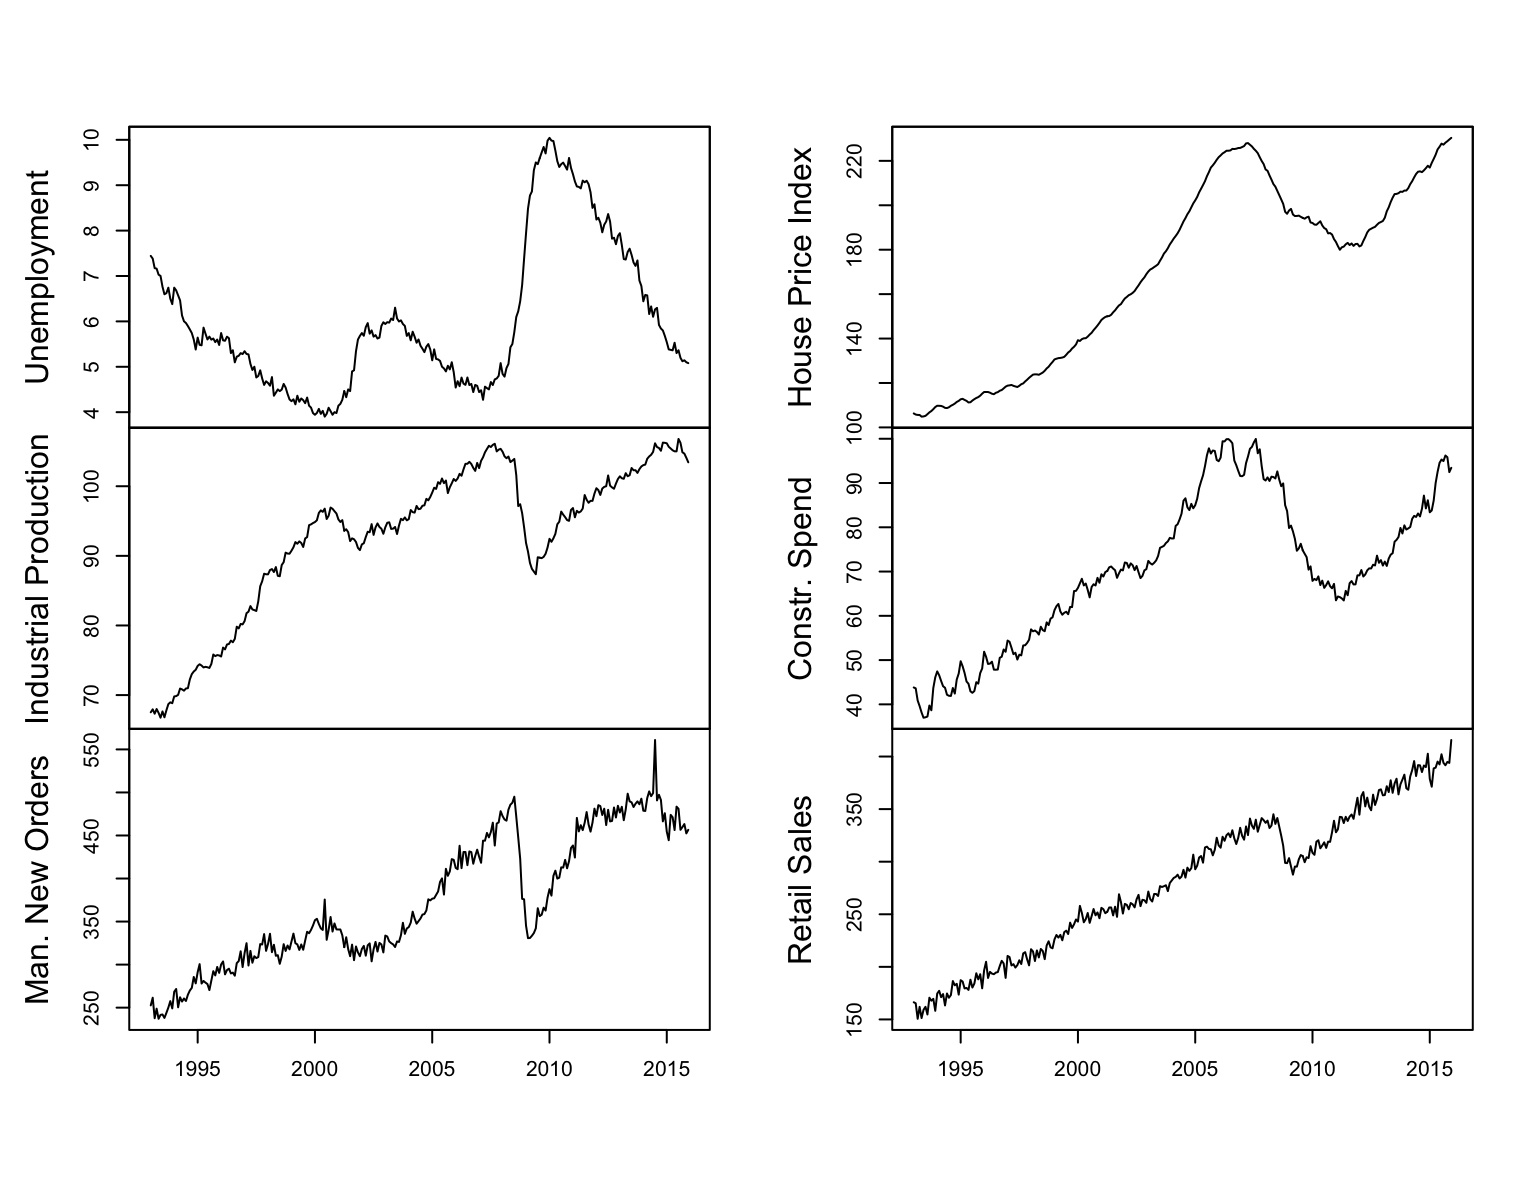
\includegraphics[width=\linewidth]{images/predictors}
\end{figure}

We also explored several predictor variables that are potentially related to unemployment.  Industrial Production measures enterprise output of the U.S. establishments \citep{BGFS2016}. Value of Manufacturers' New Orders for All Manufacturing Industries refers to manufacturer's sales and inventory, except for New Orders from the Semicondutor Industry \citep{vmno}. The Purchase Only House Price Index for the United States follows sales for a specific set of single-family homes \citep{fhfa2016}. We also included Retailers Sales \citep{retail2016} and Total Construction Spending \citep{construction2016}. Each of these predictors shows an overall increasing trend over time, see Figure \ref{fig:predictors}.
%------------------------------------------------

\section{Exploratory Analysis}
		\begin{figure}[htb]
		\centering
		\caption{Monthly unemployment, seasonally adjusted}
		\label{fig:unemployment}
		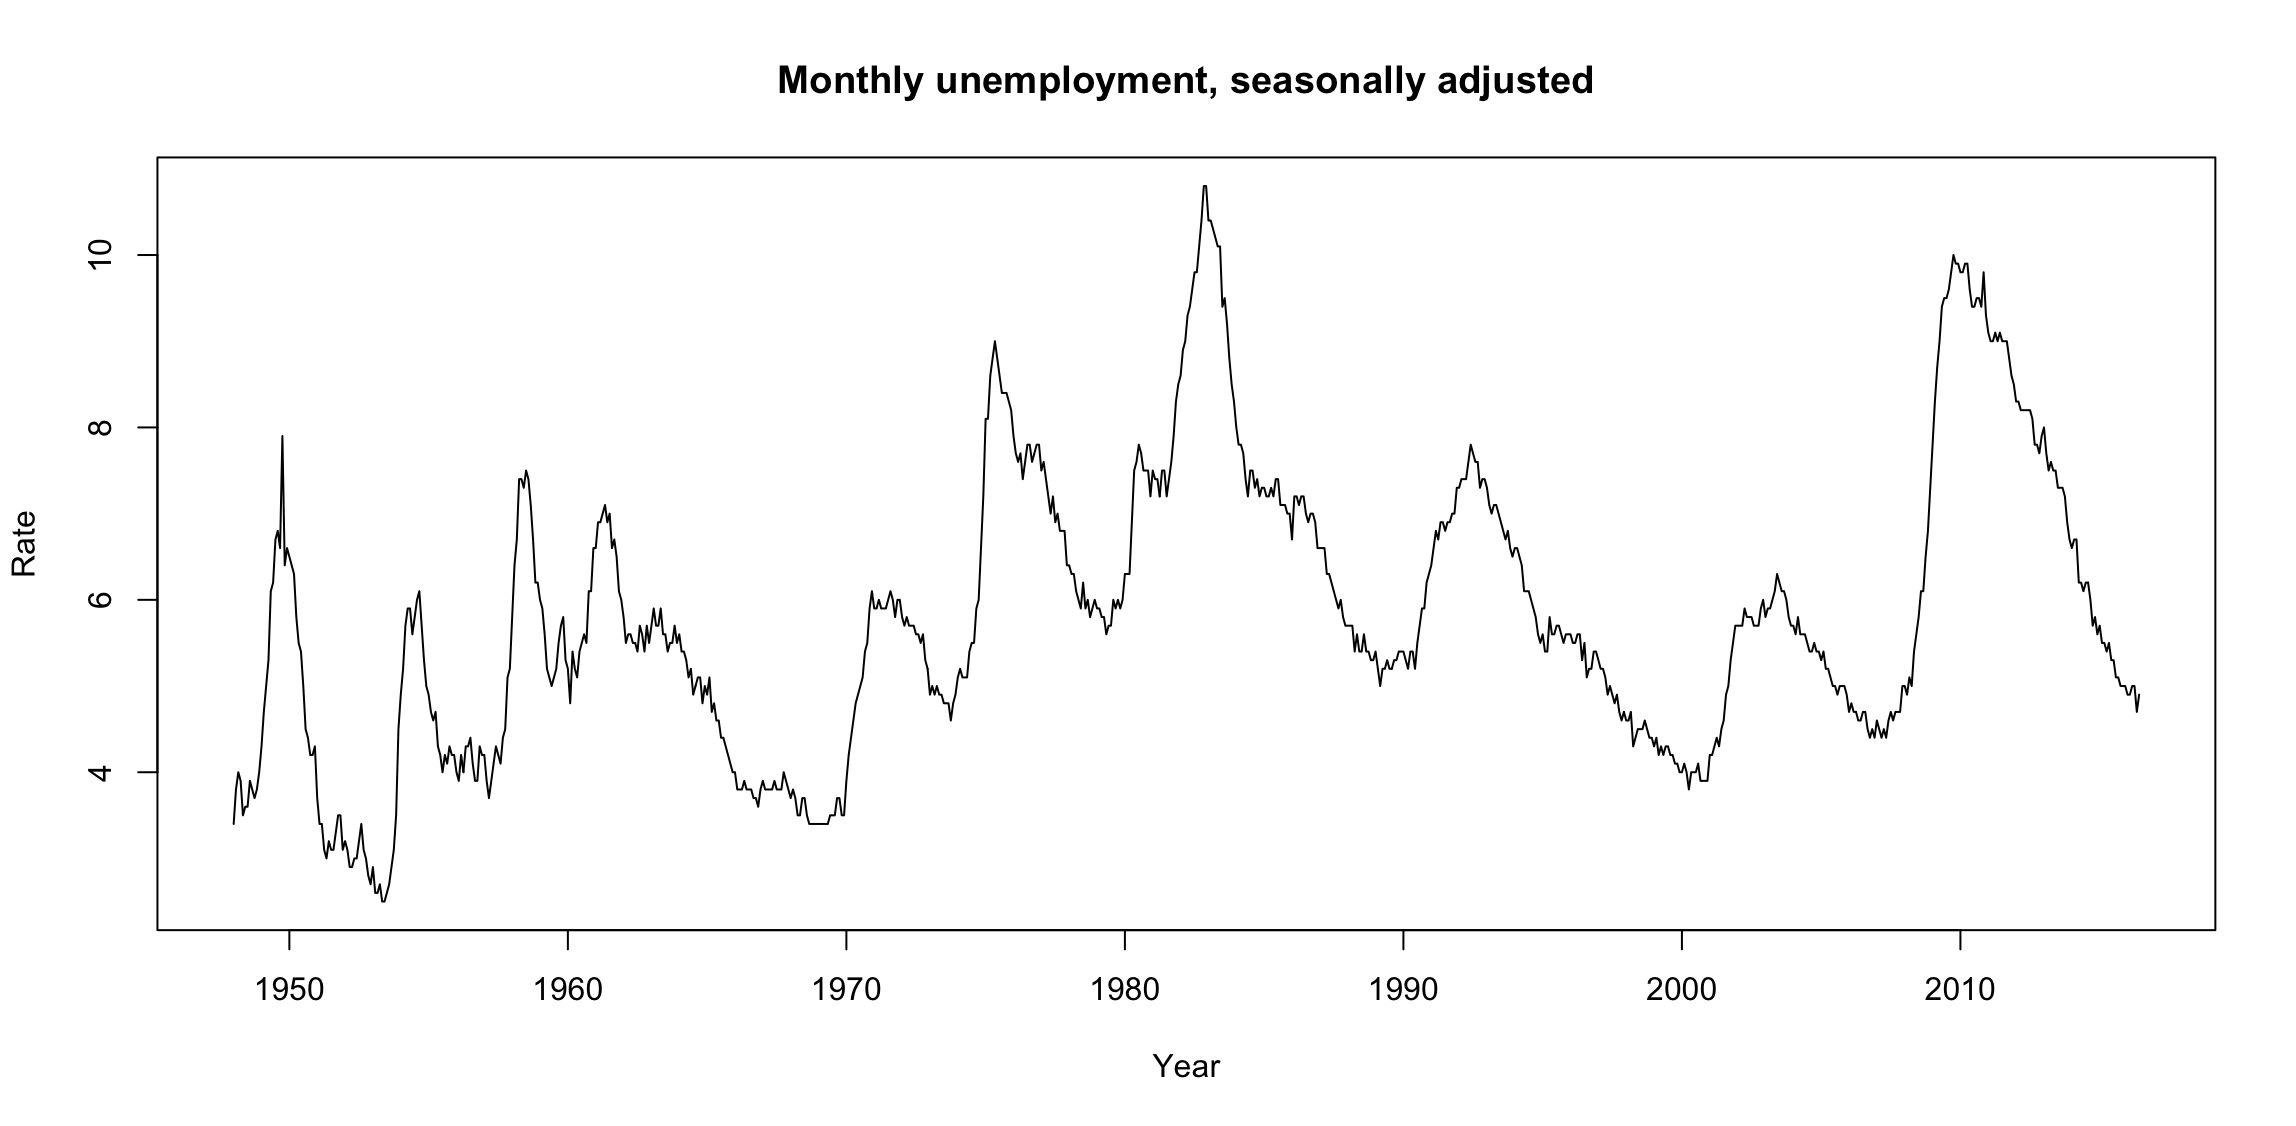
\includegraphics[width=\linewidth]{images/unemployment_total_sa}
	\end{figure}
	
				\begin{figure}[htb]
		\centering
		\caption{Seasonally Adjusted Unemployment with sitting president backdrop}
		\label{fig:presunemp}
		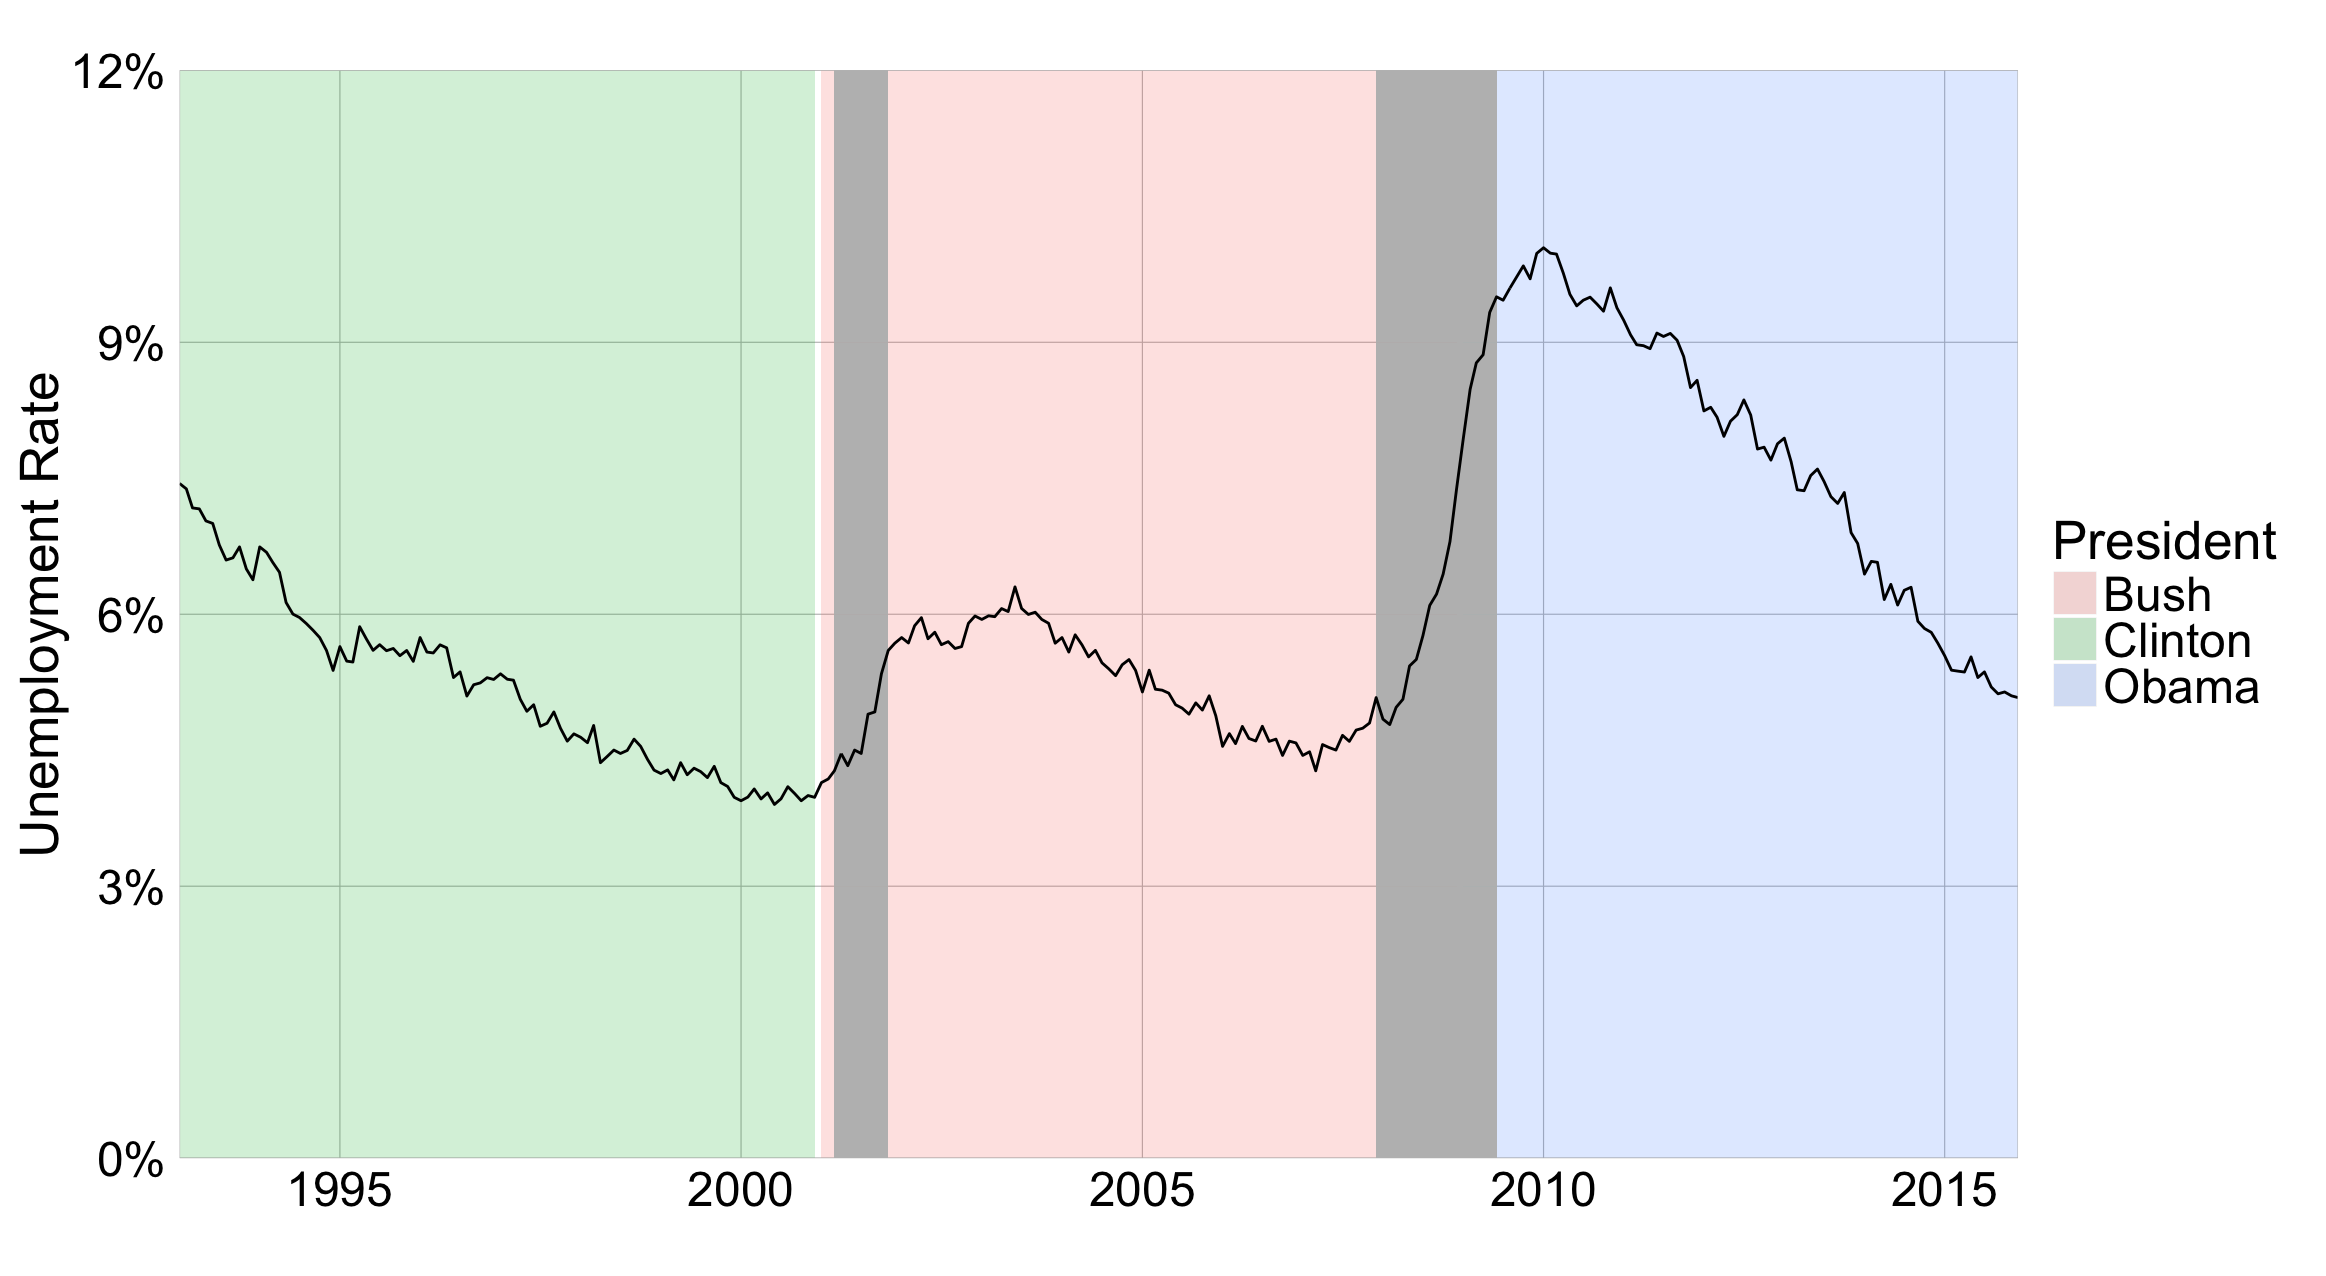
\includegraphics[width=\linewidth]{images/presunemp}
		\end{figure}


As a first step, the data was plotted over time to identify any obvious patterns visually, considering the seasonally adjusted version of the unemployment rate, see Figure \ref{fig:unemployment}.  Overall, unemployment appears relatively volatile.  There are several time periods of sudden spikes in the unemployment rate, followed by a slower recovery period. This countercyclical movement is consistent with the descriptions of unemployment data found in the literature \citep{katz2010, Montgomery1998, shimer2012reassessing}. 
	
		\begin{figure}[htb]
		\caption{Scatterplot matrix of unemployment and potential predictors}
		\label{fig:pred_scatt}
		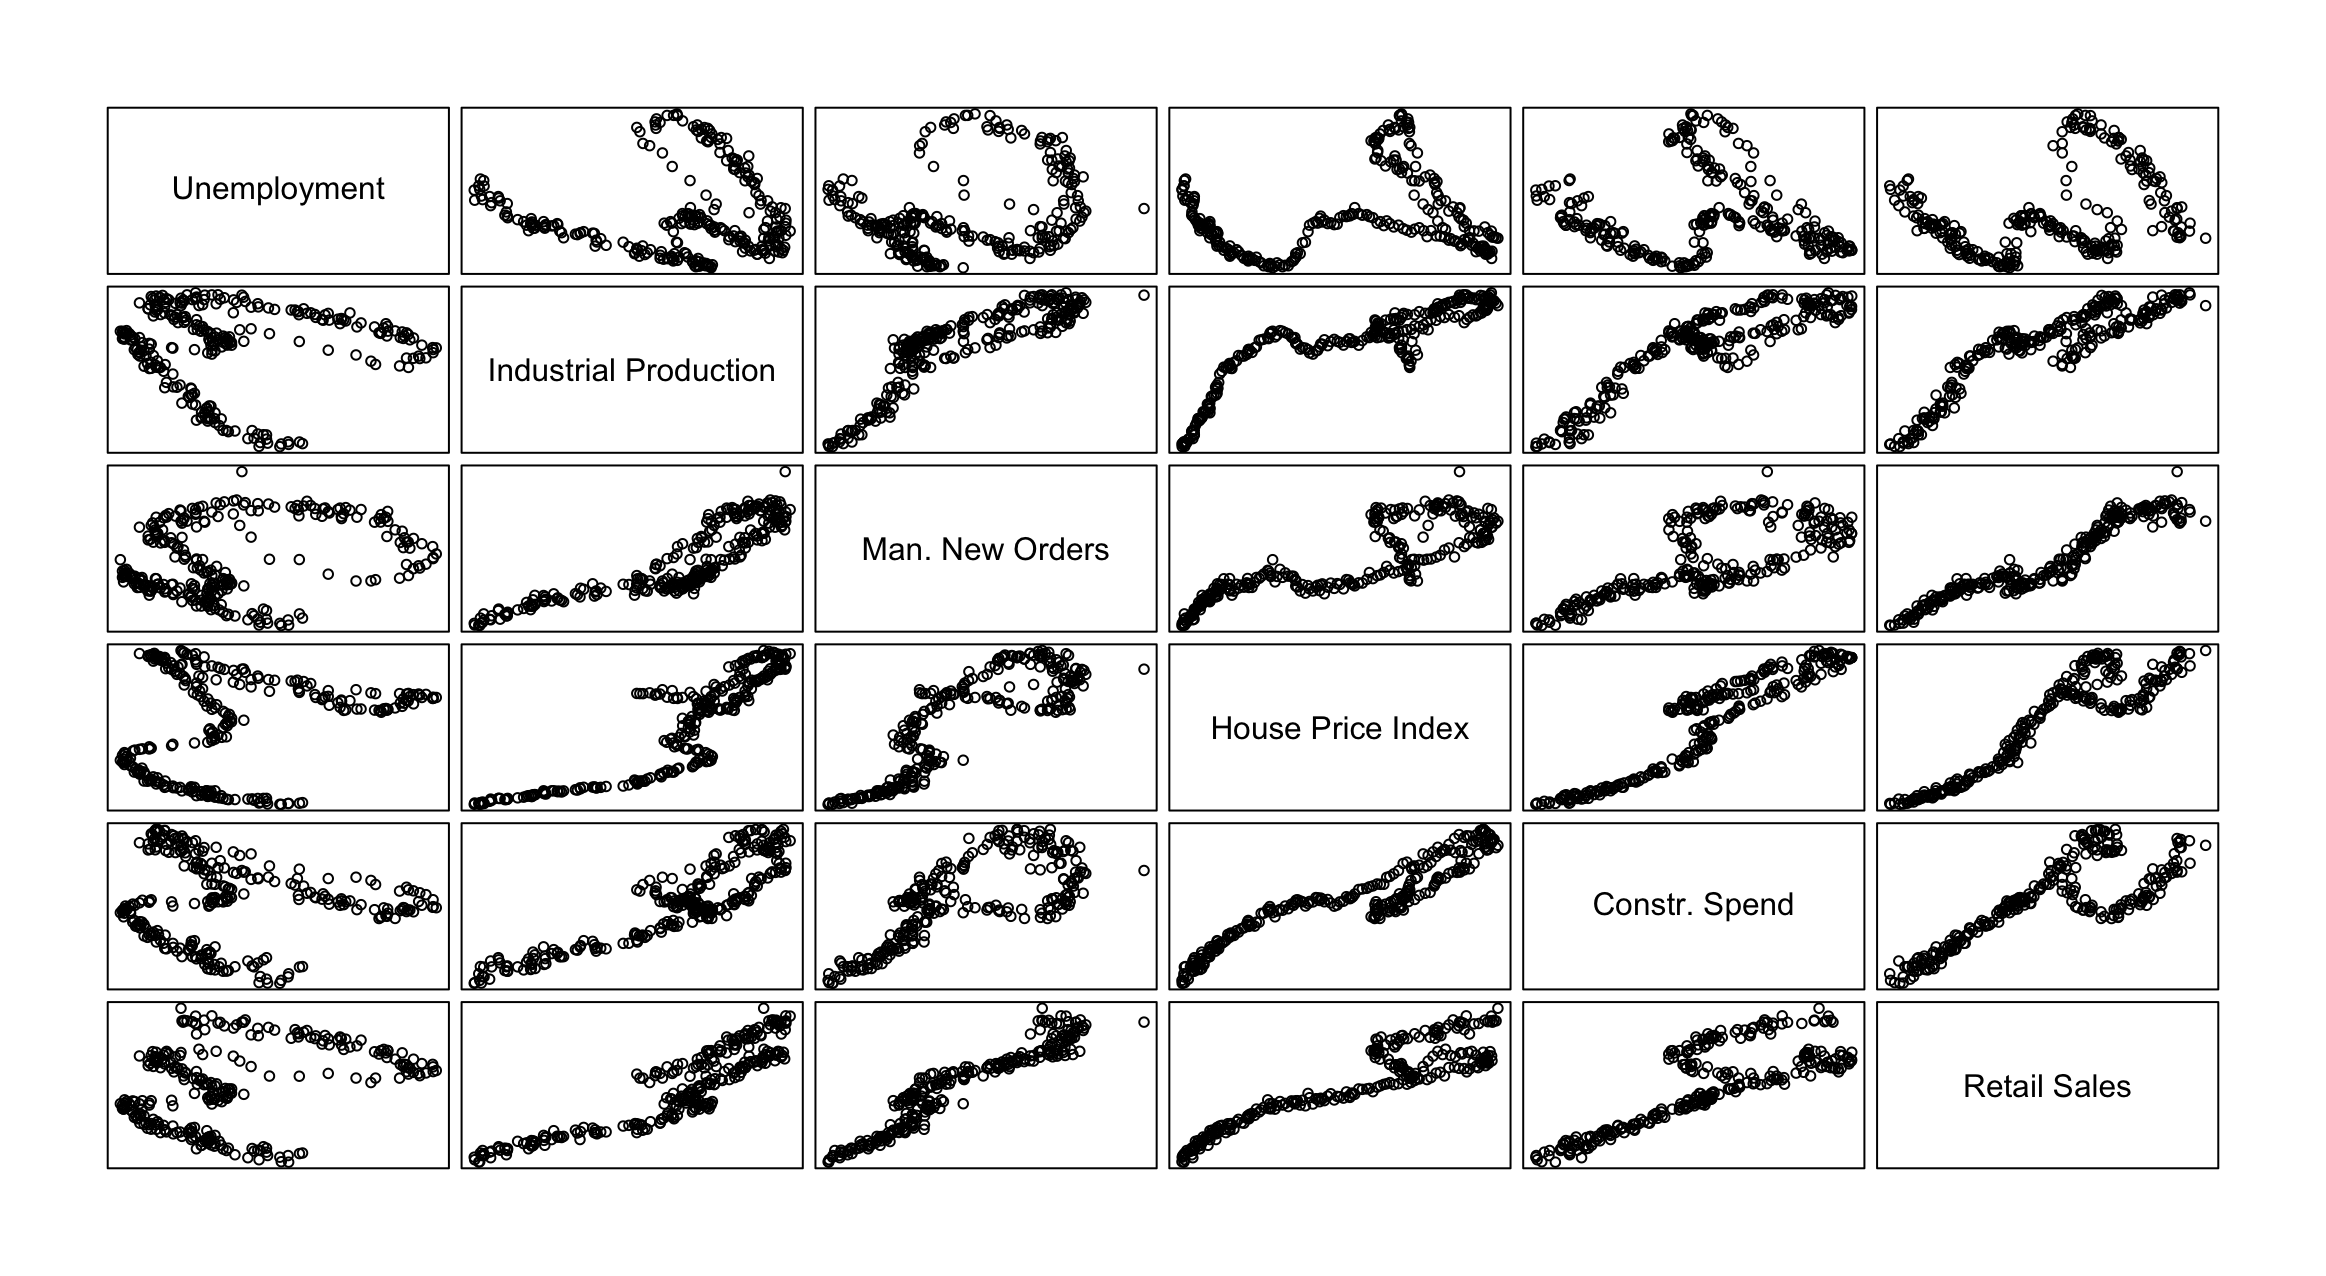
\includegraphics[width=\linewidth]{images/pred_scatt}
	\end{figure}

Due to marked potential differences in the trend surrounding times of economic downturn, such as those that occured after World War II and in the 70s and the 80s, we have chosen to limit our analysis on a more recent set of unemployment data. Ultimately, we decided to focus the time preceeding and following the Great Recession of 2007. We limited our inital analysis to 1992 to 2015, which encompases the presidential terms of Bill Clinton, George W. Bush, and Barack Obama, each serving eight years in office.  Initial graphs of the data seem to indicate that, in general, unemployment spiked at the begining of each president's term and fell gradually over the time he was in office, see Figure \ref{fig:presunemp}. There are also two noticeable spikes that represent that recessions of 2001 and 2008, respectively.  The 2008 recession also follows the burst of a housing market bubble.  These are all explanatory variables that can potentially inform unemployment patterns. A scatterplot matrix  of these predictors can be seen in Figure \ref{fig:pred_scatt}.

%------------------------------------------------

\section{Achieving Stationarity}

In analyzing the inital plots, it appears that the series could benefit from detrending. A graph of various potential lagged values for unemployment can be seen in Figure \ref{fig:laggedunemployment}. The high values of the correlation coffecients, particularly through lag 6 further suggest a high degree of autocorrelation within the unemployment dataset.    An Augmented Dickey-Fuller (ADF) test for stationarity was conducted to verify the nonstationarity of the unemployment data.  The ADF tests the null hypothesis that the time series data has a unit root against the alternative that the data are stationary \citep{Shumway2006}. The Dickey-Fuller test statistic for the unemployment data is -2.1377, with a lag order of 6, and a p-value of 0.518. The high p-values suggest that we do not have a stationary model with just the raw unemployment data.
			
		\begin{figure}[htb]
		\centering
		\caption{Autocorrelation of unemployment data}
		\label{fig:laggedunemployment}
		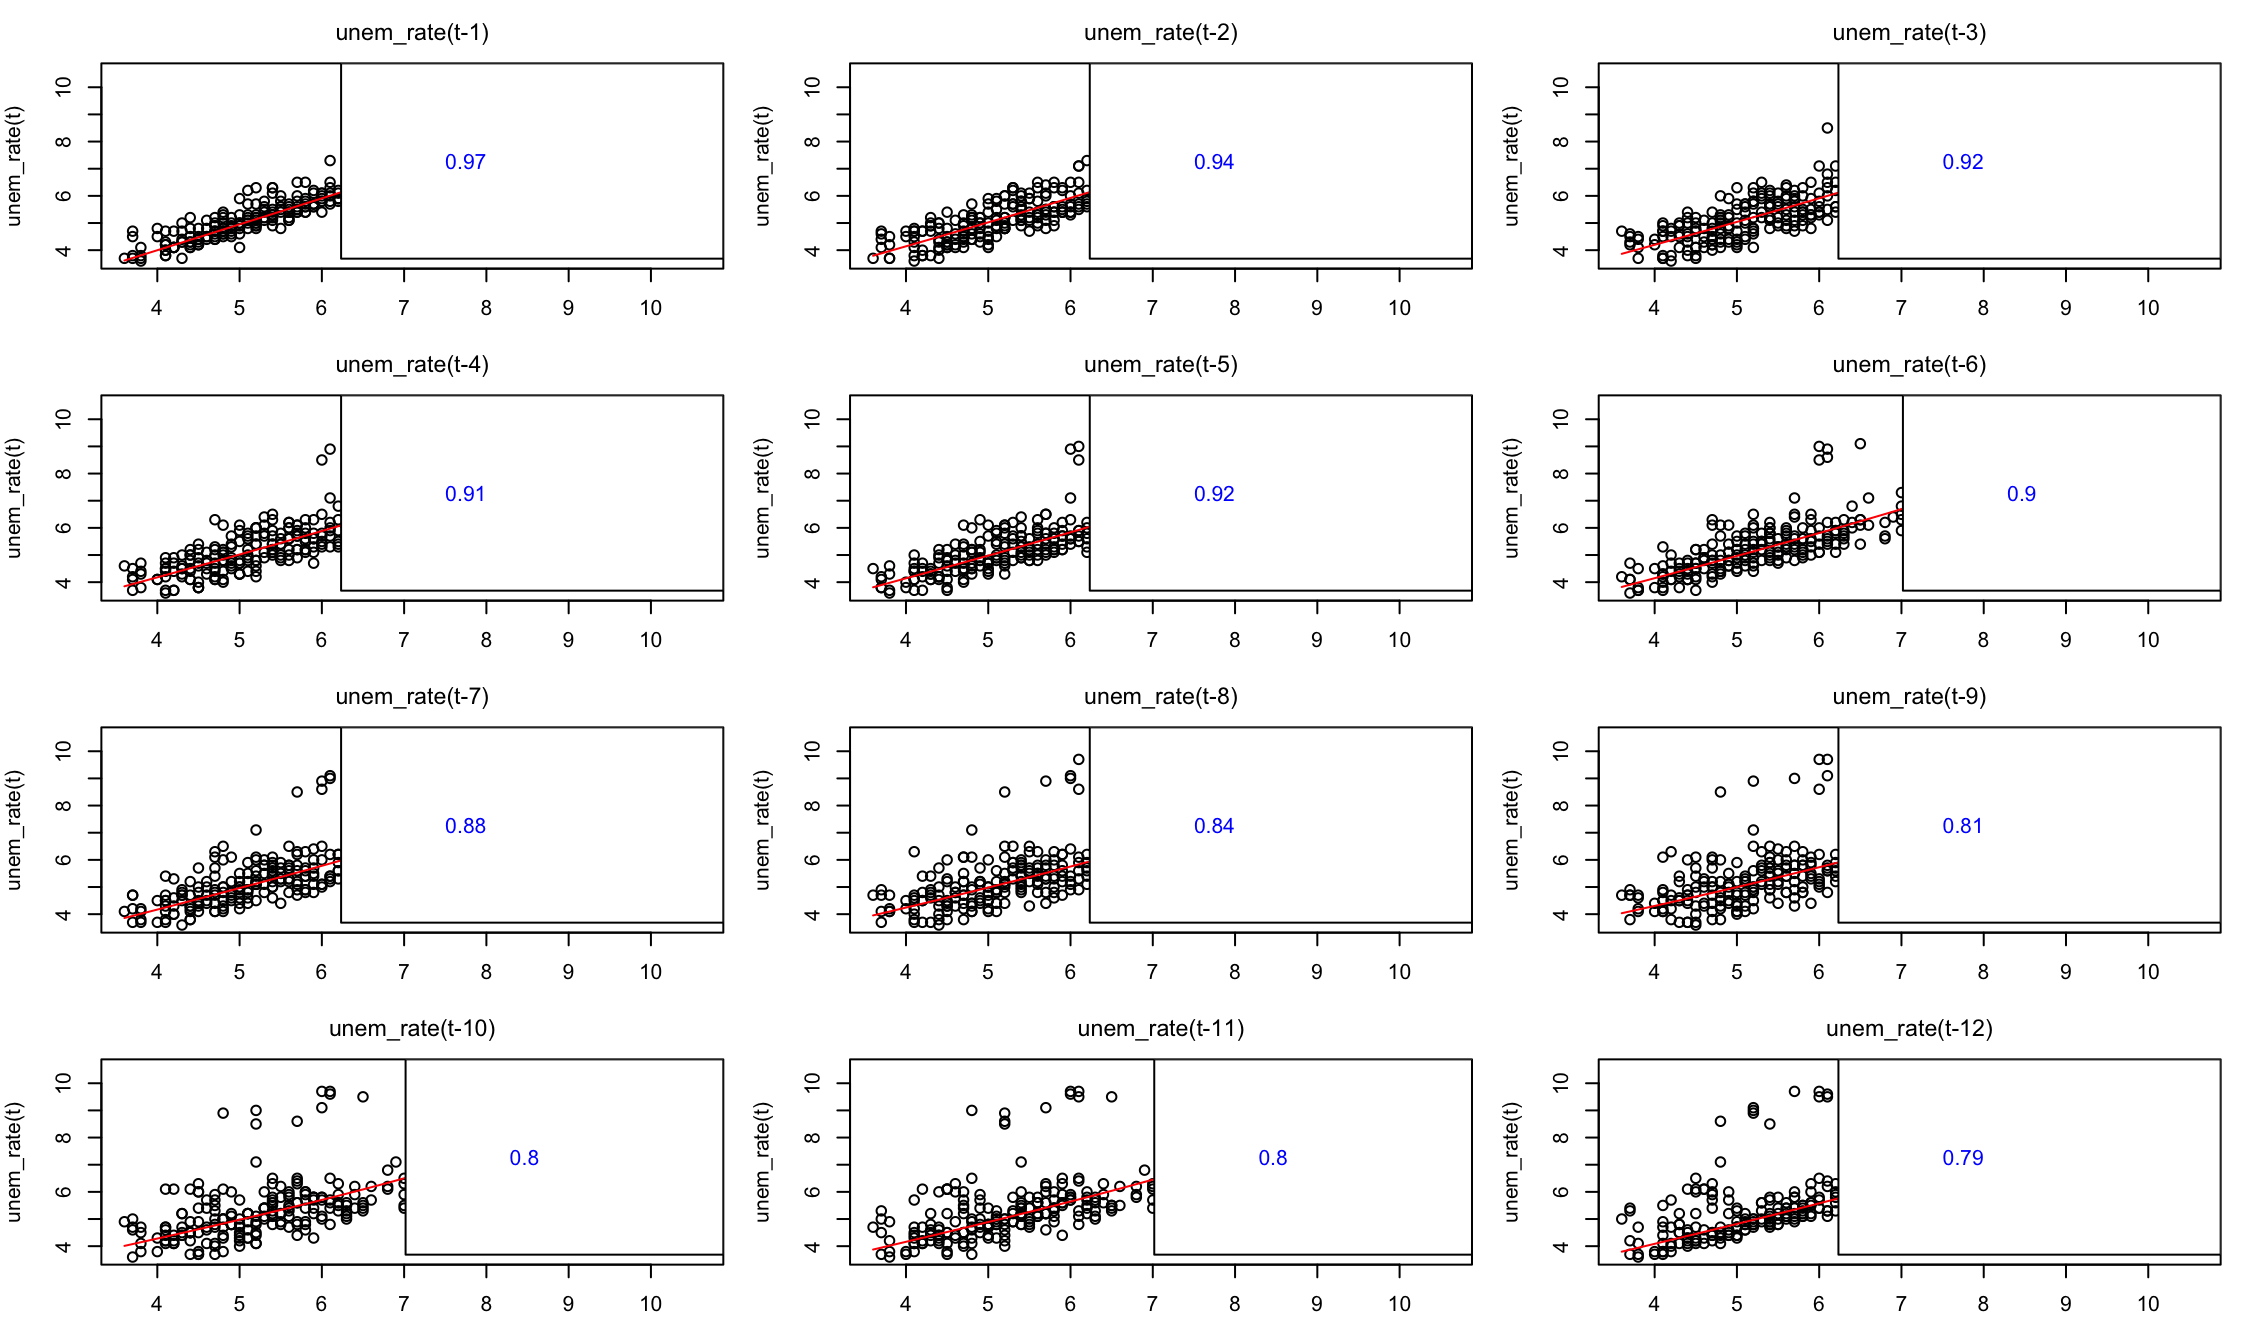
\includegraphics[width=\linewidth]{images/laggedunemployment}
	\end{figure}
The first, second, and third differences of the unemployment data were plotted for seasonally adjusted unemployment data, see Figure \ref{fig:seasonalunem}. All three sets of differencing, bring the data closer to stationarity with a consistent mean and more constant variance. The associated ADF test results are given in Table \ref{tab:ADF}. Based on the p-values, there is significant evidence of stationarity with each of the differenced models. Visually, the second differences best approximate a white noise series. Futhermore, even though the ADF statistic is more negative for the \(3^{rd}\) differences there appears to be more variability in the model that includes third differences.  Therefore, the consensus in the group was to continue the model building process using second differences.
	\begin{figure}[htb]
		\centering
		\caption{Timeplots of lagged unemployment}
		\label{fig:seasonalunem}
		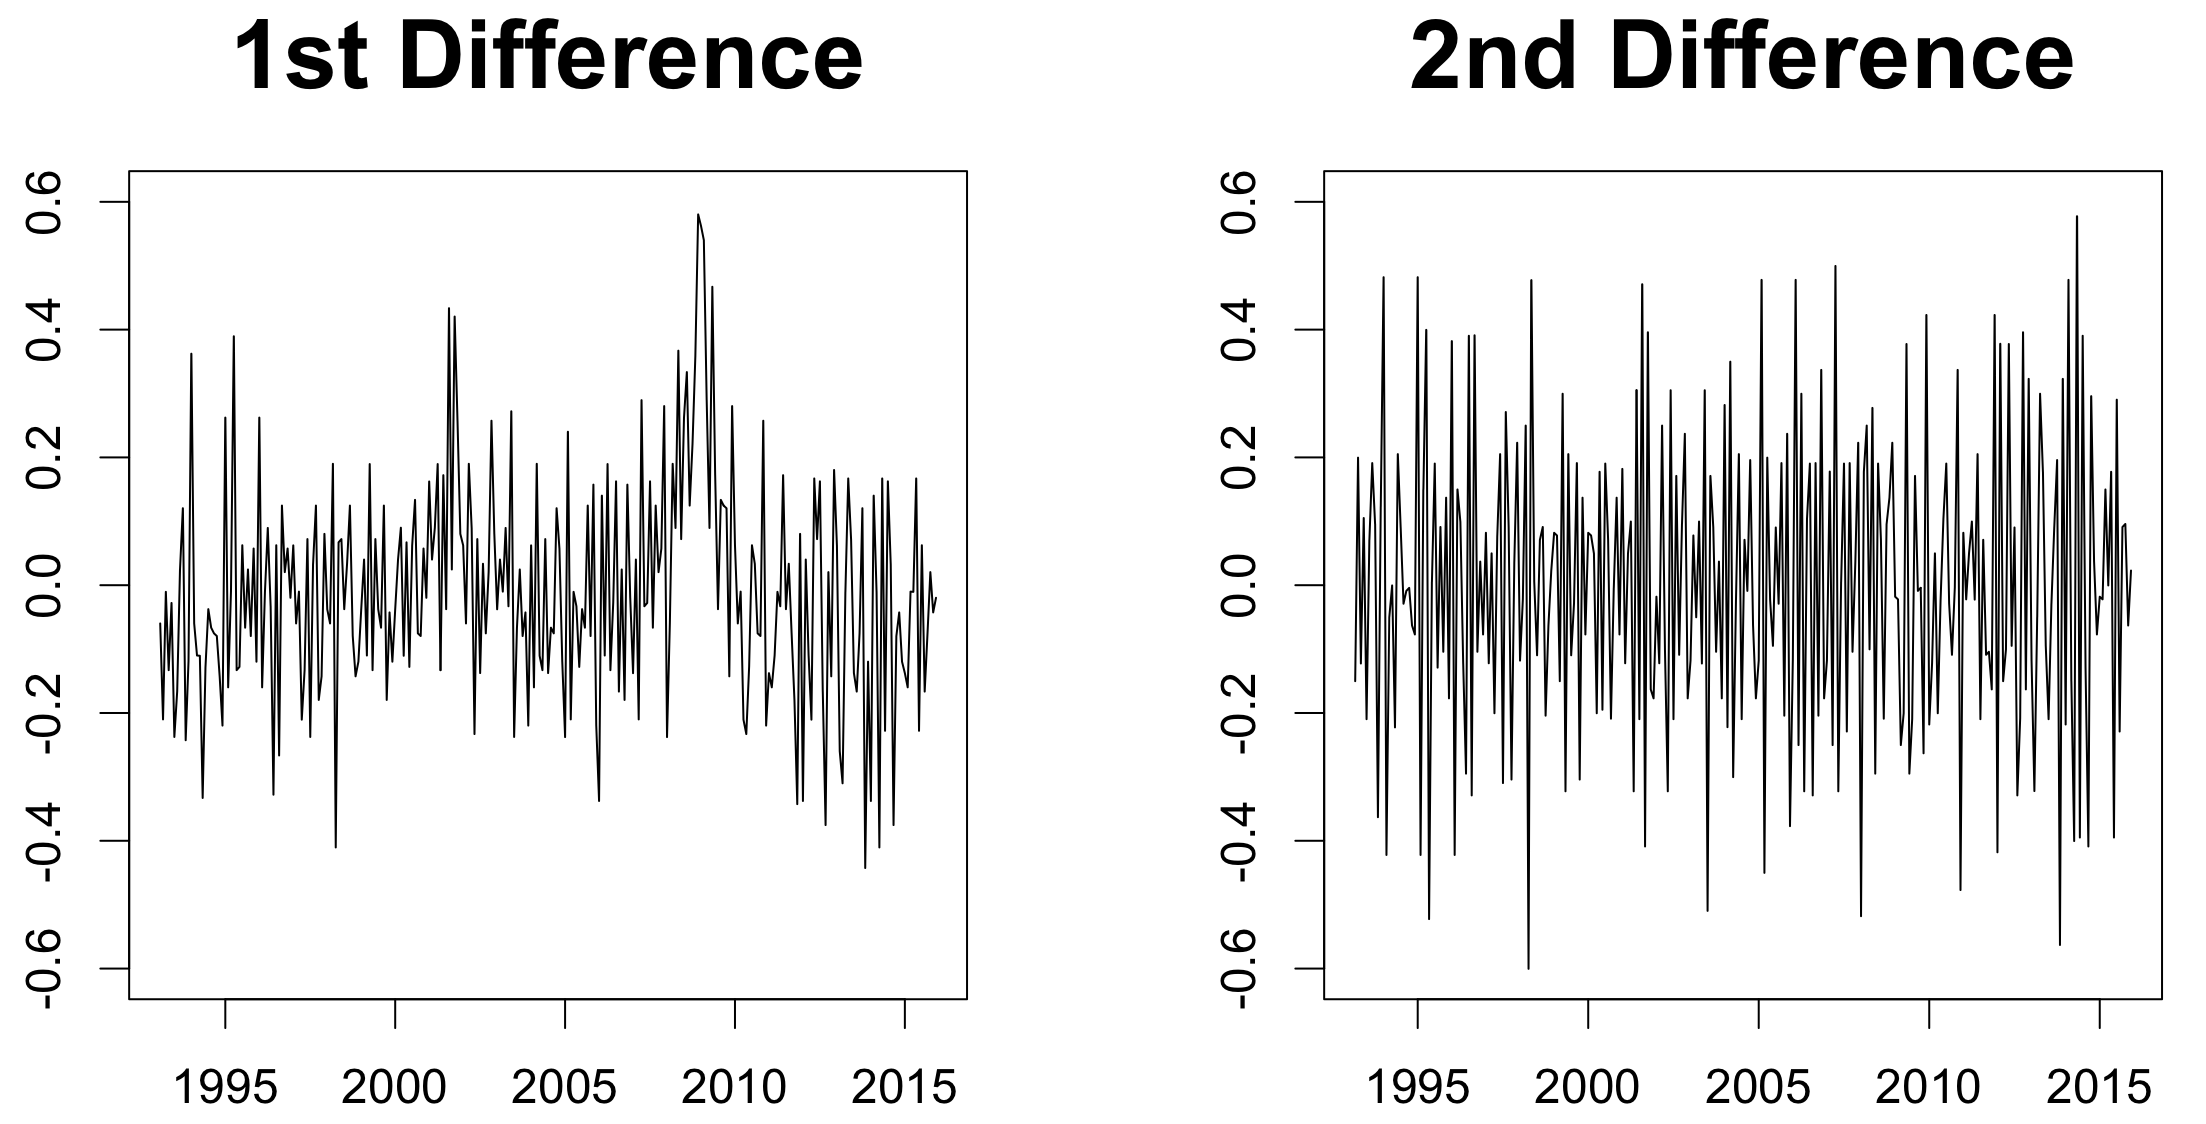
\includegraphics[width=\linewidth]{images/seasonalunem}
	\end{figure}
		 
		 \begin{table}[htb]
		 \centering
		 \caption{ADF Test Results for unemployment}
		 \label{tab:ADF}
		 \begin{tabular}{lllll}
		 \hline
		 \textbf{Model} & \textbf{Statistic} & \textbf{Lag order} & \textbf{p-value}\\ \hline
		  1\(^{st}\) difference &  -9.3595 & 6 &\( < 0.01\)\\
		  2\(^{nd}\) difference &  -9.3595 & 6 & \( < 0.01\)\\			  
		  3\(^{rd}\) difference &  -13.02 & 6 & \( < 0.01\)\\		 \hline
		 \end{tabular}
		 \end{table}
The predictor variables were also detrended using second differences. The timeplots of these second differences can be seen in Figure \ref{fig:statpred}. Although the housing prices still retains some nonconstant variance, overall the differencing improves the stationarity of all the predictor variables.  Futhermore, the ADF test of the differenced data provides evidence of stationarity for each of the variables, See table \ref{tab:ADF2}. 

		\begin{figure}[htb]
		\centering
		\caption{Timeplots of differenced predictors}
		\label{fig:statpred}
		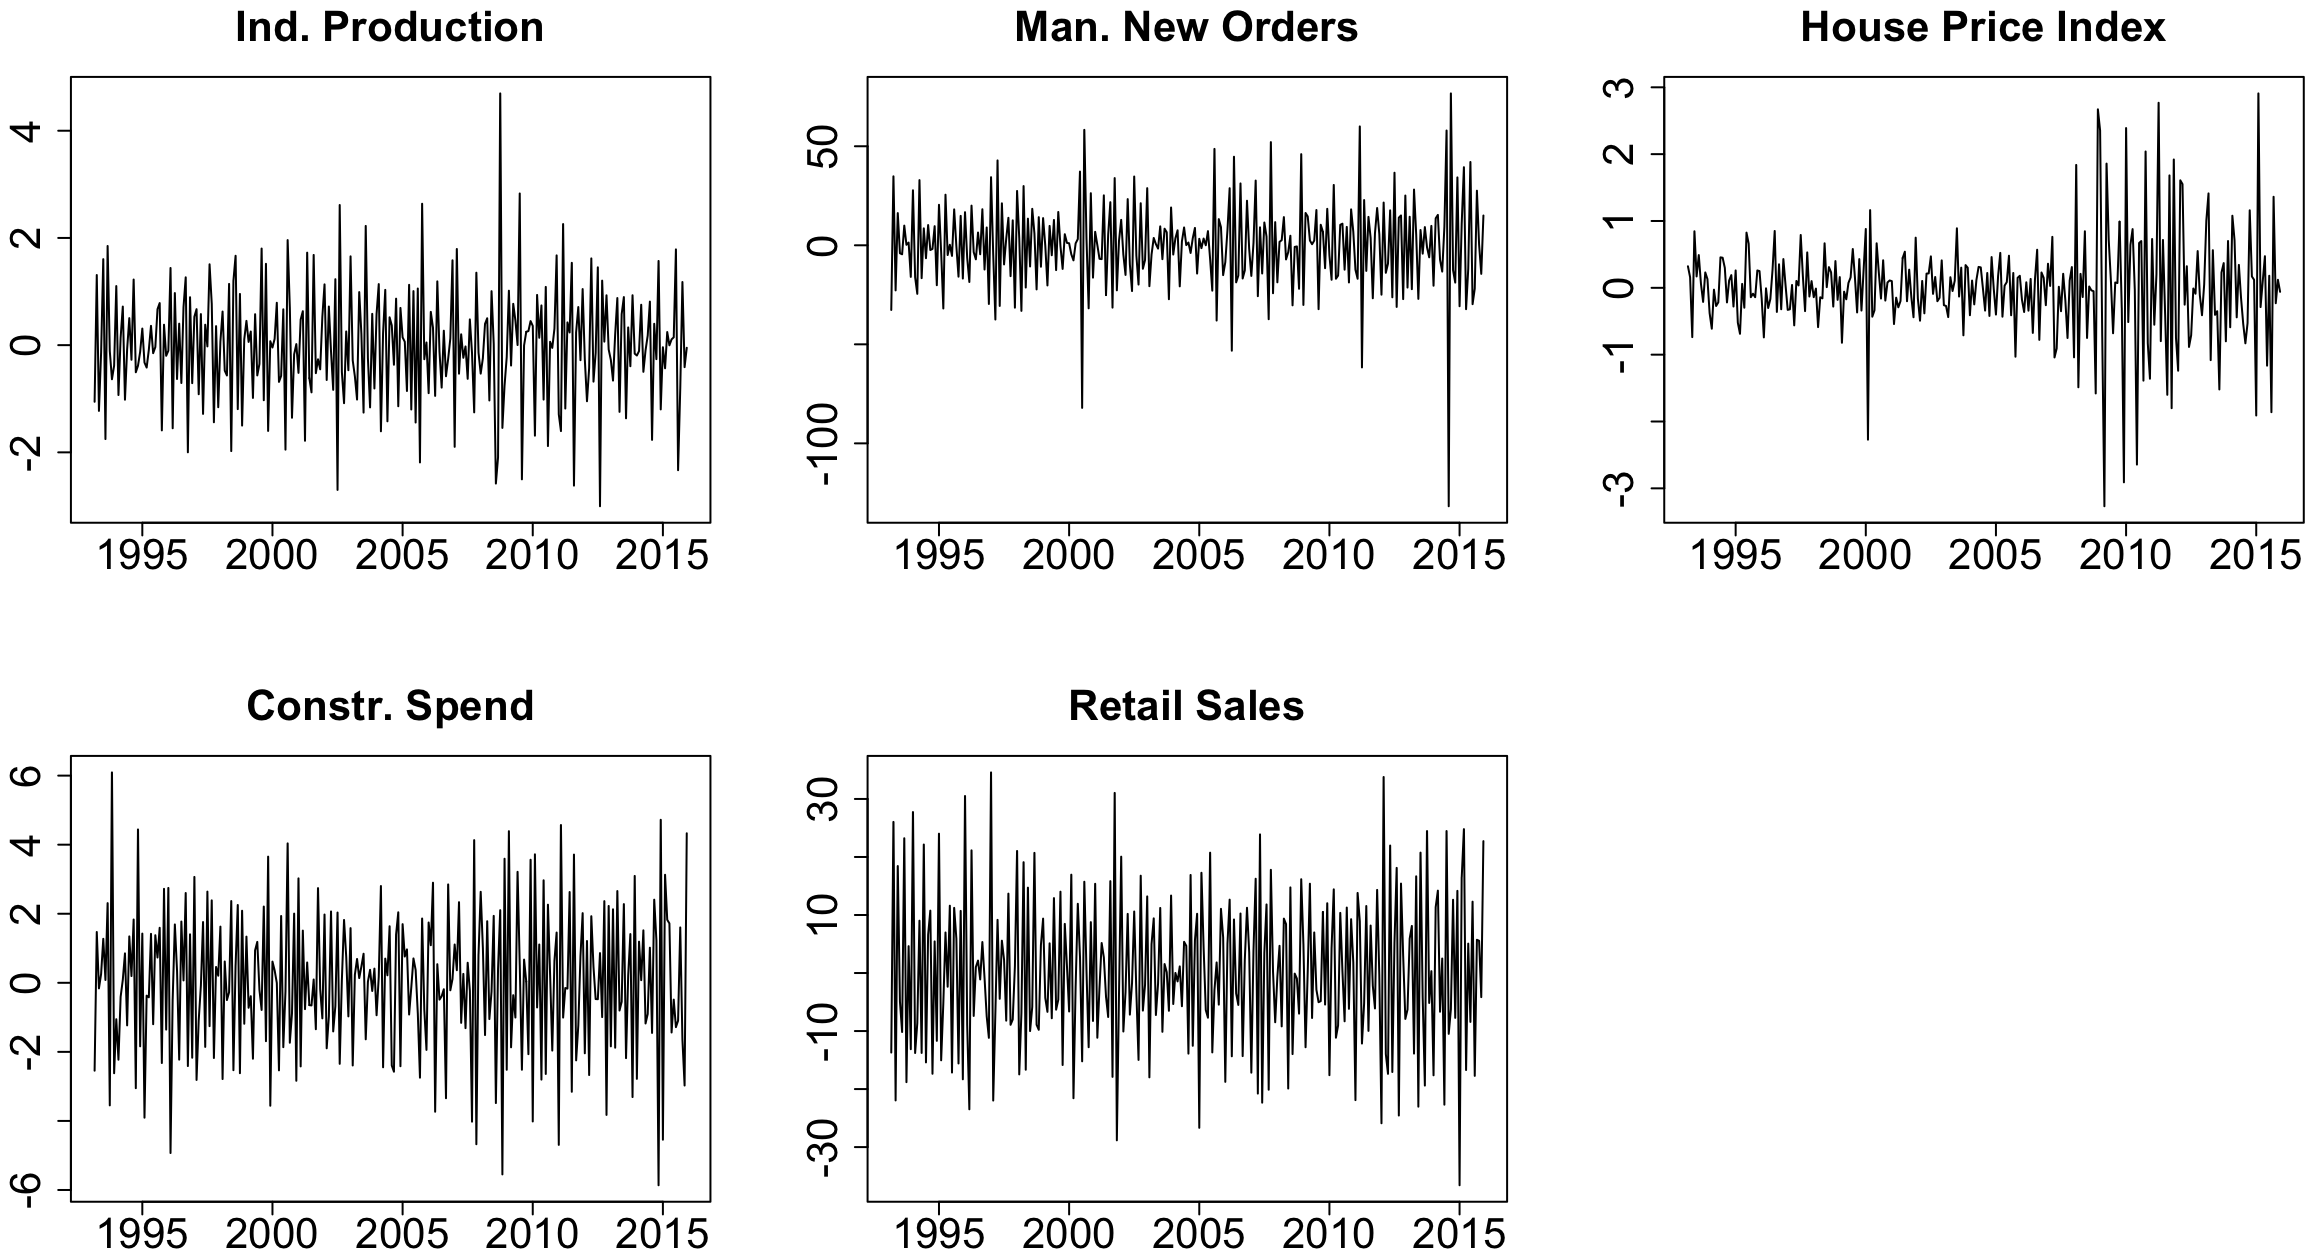
\includegraphics[width=\linewidth]{images/StationaryPred}
		\end{figure}

An attempt to stabalize the variance of the housing prices, utilizing a log transform, does not improve this stationarity much (ADF changes from -9.104 to -9.5211 and a scatterplot of the differenced logs still shows evidence of heteroscedasticity in the variance over time, see Figure \ref{fig:loghouse}. 


		
		\begin{figure}[htb]
		\centering
		\caption{Timeplot of transformed housing prices, d=2}
		\label{fig:loghouse}
		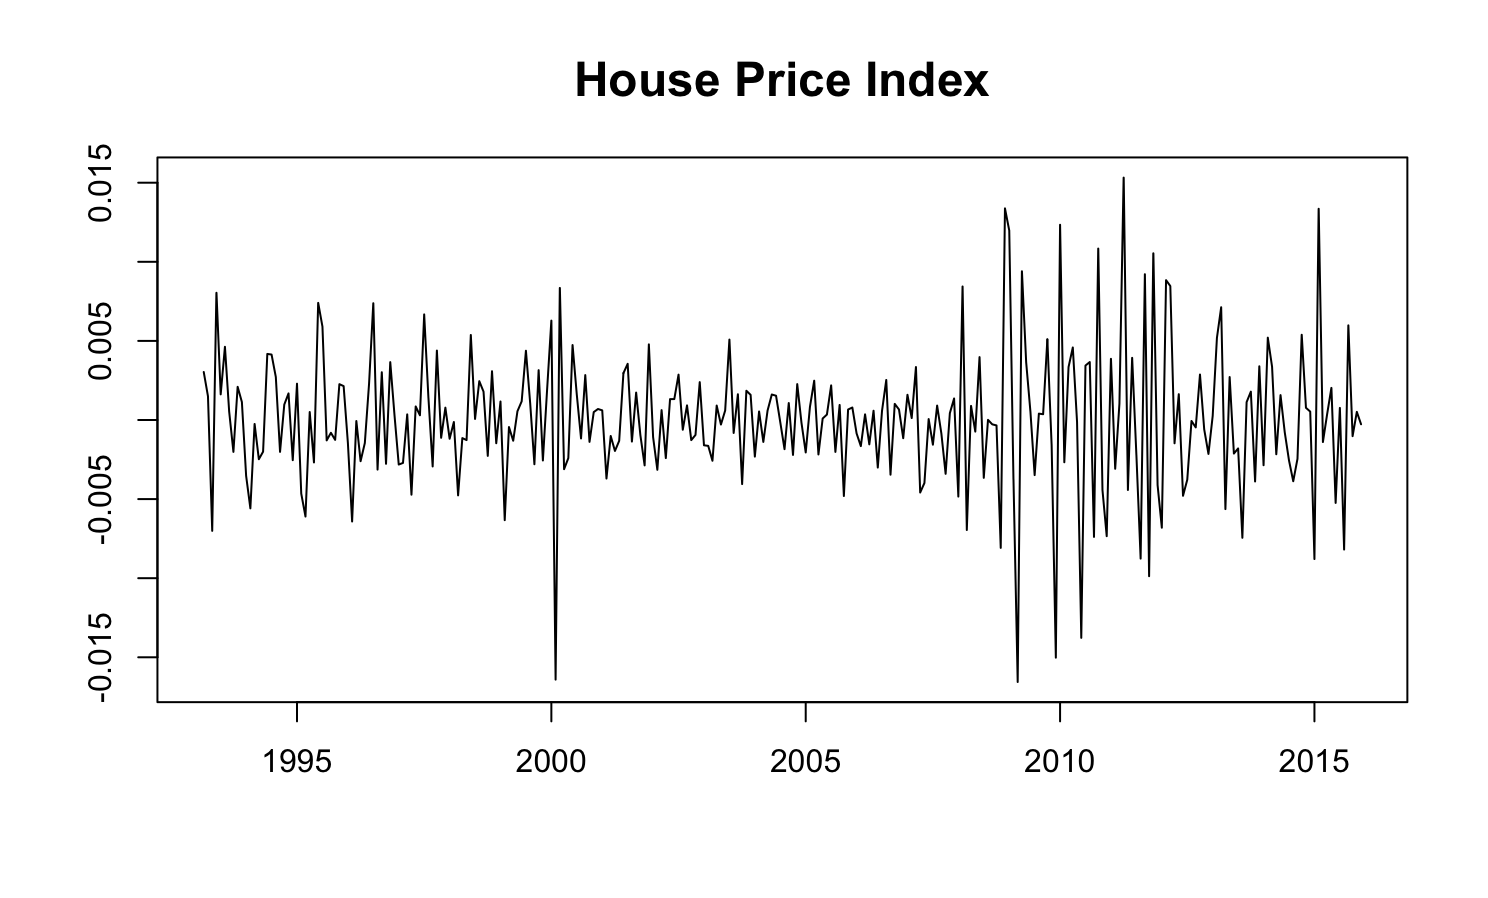
\includegraphics[width=\linewidth]{images/houseprice}
	\end{figure}


		 
\begin{table}[htb]
		 \centering
		 \caption{ADF Test Results for Predictors, \(d=2\)}
		 \label{tab:ADF2}
		 \begin{tabular}{lllll}
		 \hline
		 \textbf{Variable} & \textbf{Statistic}  & \textbf{p-value}\\ \hline
		  Industrial Production & -9.2333  &\( < 0.01\)\\
		  New Orders &  -8.391  & \( < 0.01\)\\			  
		  House Prices &  -9.104  & \( < 0.01\)\\				  
		  Construction Spending &  -10.447 &  \( < 0.01\)\\
		  Retail Sales &  -10.72 &  \( < 0.01\)\\ \hline
		 \end{tabular}
		 \end{table}

	 

  


%------------------------------------------------

\section{Model Building}

 
    \begin{figure}[hbt]
    	\centering
     	\caption{ACF \& PACF Plots}
     	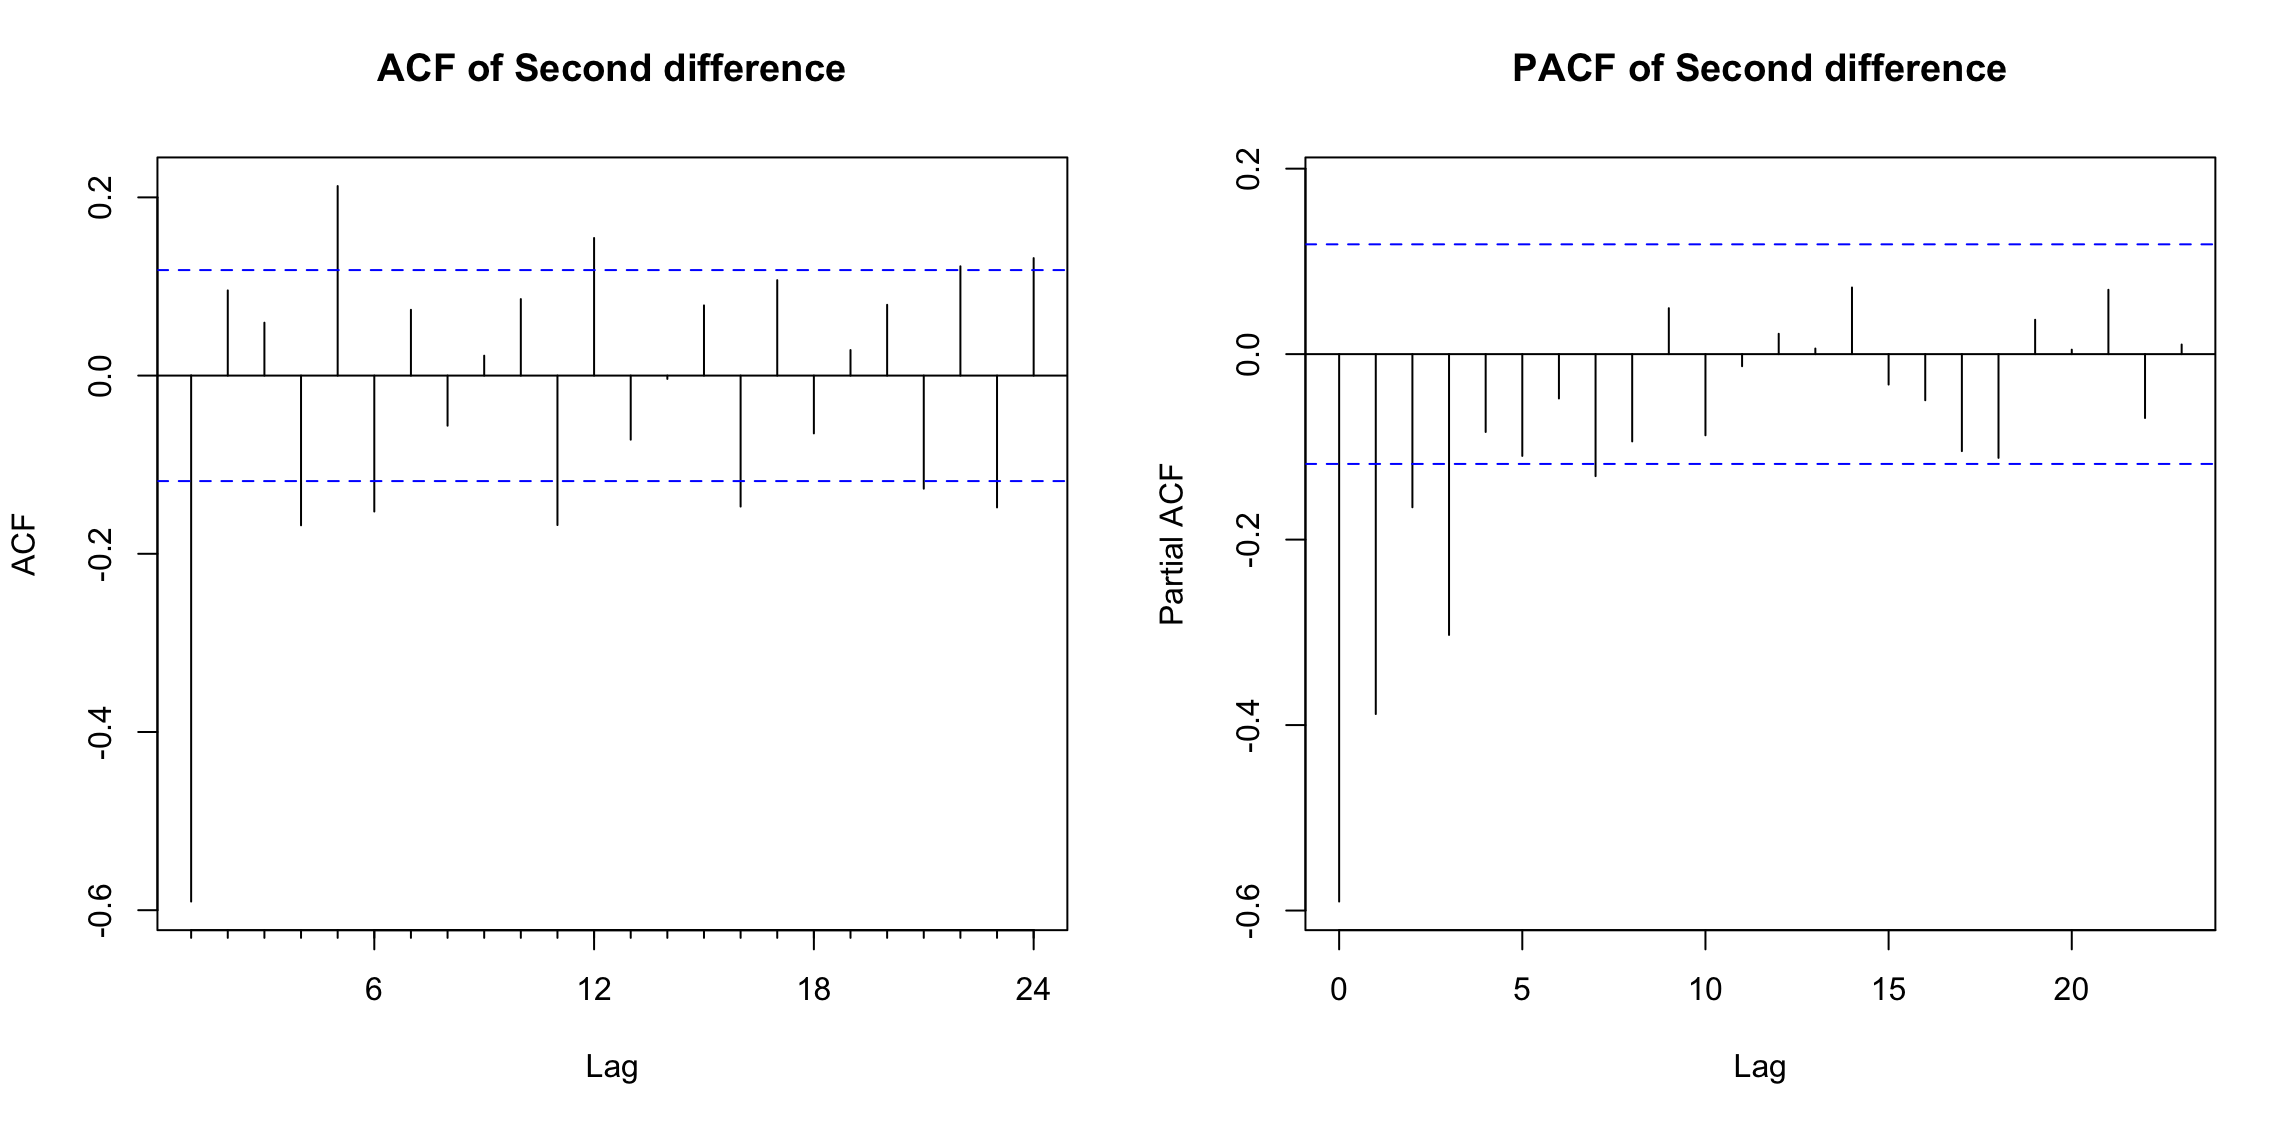
\includegraphics[width=\linewidth]{images/acfpacf}
     	\label{fig:acfpacf}
     	\caption{ACF \& PACF Plots of Second Differences}
     	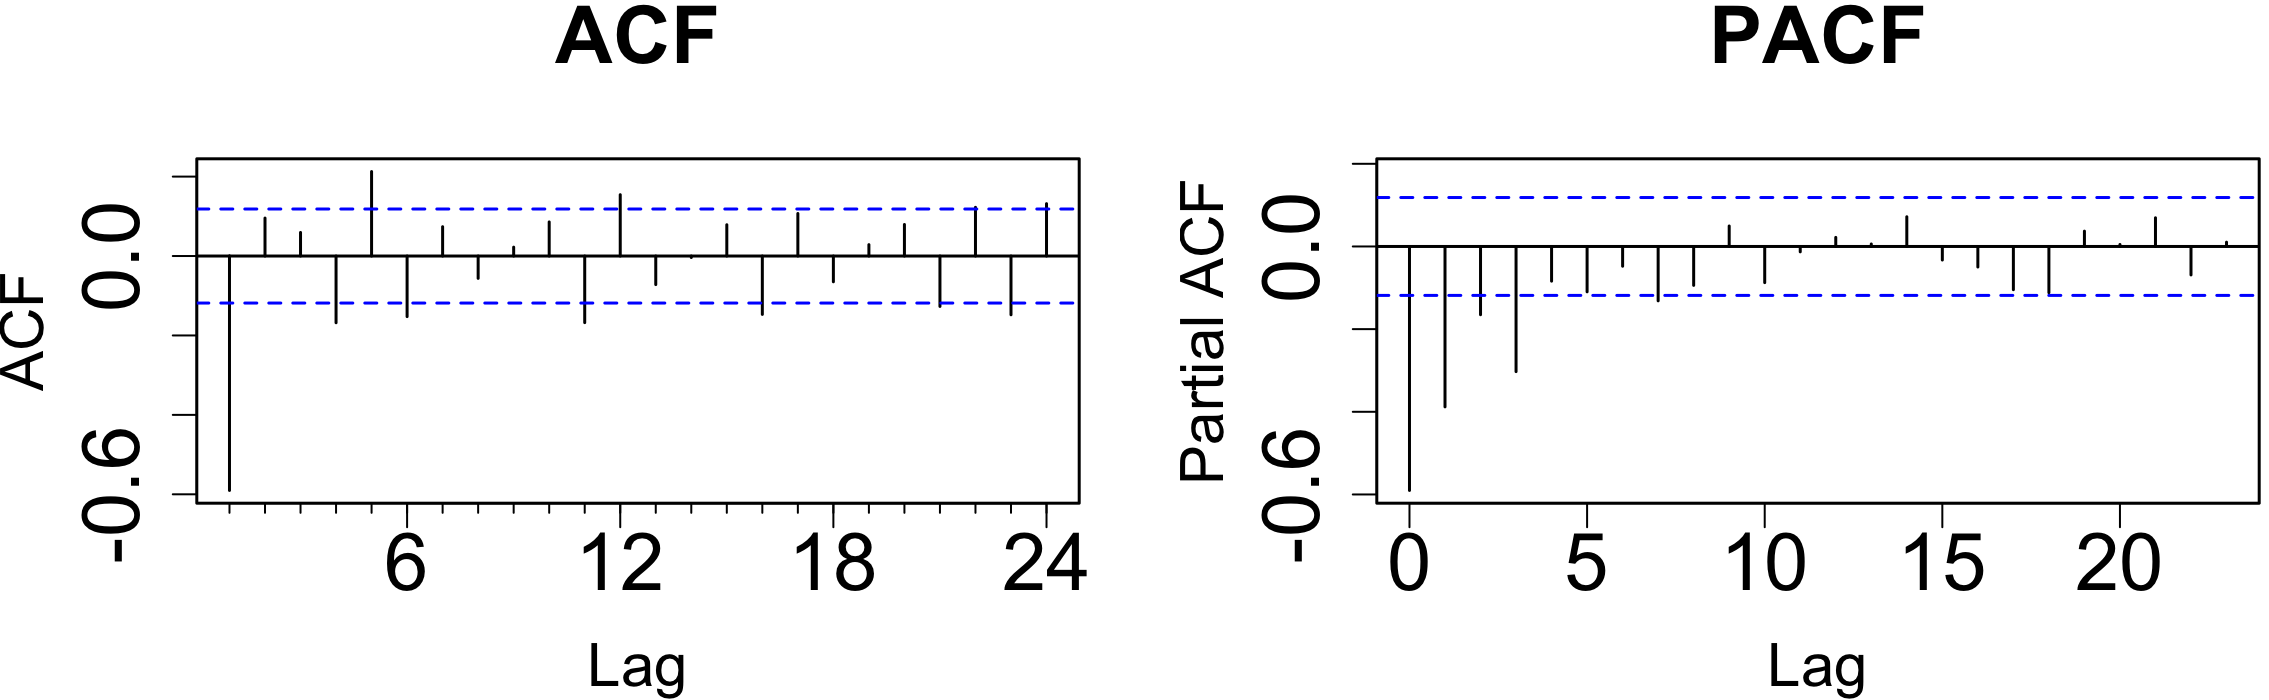
\includegraphics[width=\linewidth]{images/acfpacf2d}
     	\label{fig:acfpacf2}
      \end{figure}

  We began our model building process by inspecting the correlogram (ACF plot) and partial correlogram (PACF plot) of the unemployment data, see Figure \ref{fig:acfpacf}. The ACF seems to tail off and the PACF seems to cut off at either 1 or 3.  A tailing ACF function with a PACF that cuts off at \(p\) suggests an AR(\(p\)) model \citep{Box2008}. Therefore, these inital plots suggest a possible AR(1) or AR(3) model. When looking at the ACF and PACF of the second differences, we have evidence of a possible mixture model with \(d=2\). For example, an ACF of difference \(d\) that decays exponentially after lag 1 with a PACF that is dominated by an exponential decay pattern after lag 1 would be evidence of an ARIMA(1,\(d\),1) model . Therefore, it is worthwhile considering ARIMA models such as ARIMA(1,2,1). Of course predictor variables may help to improve the predictive strength of our models, therefore models with regressors and Vector Autogressive Models (VAR) were considered as well.

\subsection{Models Considered}
%I think we should remove the code fragment and just show the tables. We could always refer to our github project (which I can clean up) as the source for our code so people can see what functions we actually used. Also notice that the AIC in the table is different from the AIC extracted with the code. I noticed that the SARIMA produces multiple AIC, so I used the AIC extraction function to pull it out of the model frame at a lower level in the output object. I think this was better because it matches up with the same technique used in the VAR model.

\subsubsection{ARIMA Models}
% latex table generated in R 3.3.1 by xtable 1.8-2 package
% Sun Jul 24 08:35:48 2016
\begin{table}[htb]
\centering
\caption{ARIMA models considered}
\label{tab:arimachoices}
\begin{tabular}{cllrrl}
  \hline
 Model & Order & Reg  & AIC & BIC & Best \\ 
  \hline
1 & 1,2,1 &  NA &   -212.30 & -201.46 & BIC \\ 
  2  & 2,2,2 & NA   & -211.81 & -193.74 &  \\ 
  3  & 3,2,3 &  NA  & -215.48 & -190.19 &  \\ 
  4  & 1,2,1 & X  & -211.56 & -182.65 &  \\ 
  5  & 2,2,2 & X   & -209.83 & -177.32 &  \\ 
  6  & 3,2,3 & X   & -215.10 & -171.74 &  \\ 
  7  & 1,2,1 &  LagX & -222.45 & -193.69 & AIC \\ 
  8  & 2,2,2 &  LagX & -220.70 & -188.35 &  \\ 
  9  & 3,2,3 &  LagX & -217.89 & -174.76 &  \\ 
   \hline
\end{tabular}
\end{table}

Given the potenial of ARIMA models to represent the unemployment data we began by exploring three potential models without regressors, ARIMA(1,2,1), ARIMA(2,2,2), and ARIMA(3,2,3). Although model 3, ARIMA(3,2,3), has the lowest AIC of the three models, model 1, the ARIMA(1,2,1) model, has the lowest BIC. Model 1 is also the most parsimonious model of the three. So of the three intitial models, without regressors, we chose to retain model 1.  

The univariate ARIMA models we began with seem to fit the data well and have the added strength of being relatively simple models. Nevertheless, in their simplicity univariate models are not equiped to accurately portray the asymmetric nature of unemployment data and have a tendency of underpredicting during economic slowdowns \citep{Montgomery1998}. Therefore, we repeaded the above analysis using multivariate ARIMA models.  The variables Industrial Production, Value of Manufacturers' New Orders, Purchase Only House Price Index,  Retailers Sales, and Total Construction Spending were includedpotential predictors of unemployment. 

Models 4 through 6 were ARIMA(1,2,1), ARIMA(2,2,2), and ARIMA(3,2,3) respectively.  These predictors had lower AIC and BIC values than their original counterparts without regressors, see Table \ref{tab:arimachoices}. Since, these models were predicting a lagged response variable using data that was potentially nonstationary, we chose to repeat the process using lagged regressors.  Models 7, 8, and 9 refer to the ARIMA(1,2,1), ARIMA(2,2,2), and ARIMA(3,2,3) models with lagged predictor variables.  Of these three new models, model 7 has both the smallest AIC and the smallest BIC values. In fact of all 9 of our original models, model 7 has the lowest AIC overall, see Table \ref{tab:arimachoices}.  


		    \begin{figure}[htb]
    	\centering
    	\caption{Model 7: Residual Diagnostics}
     	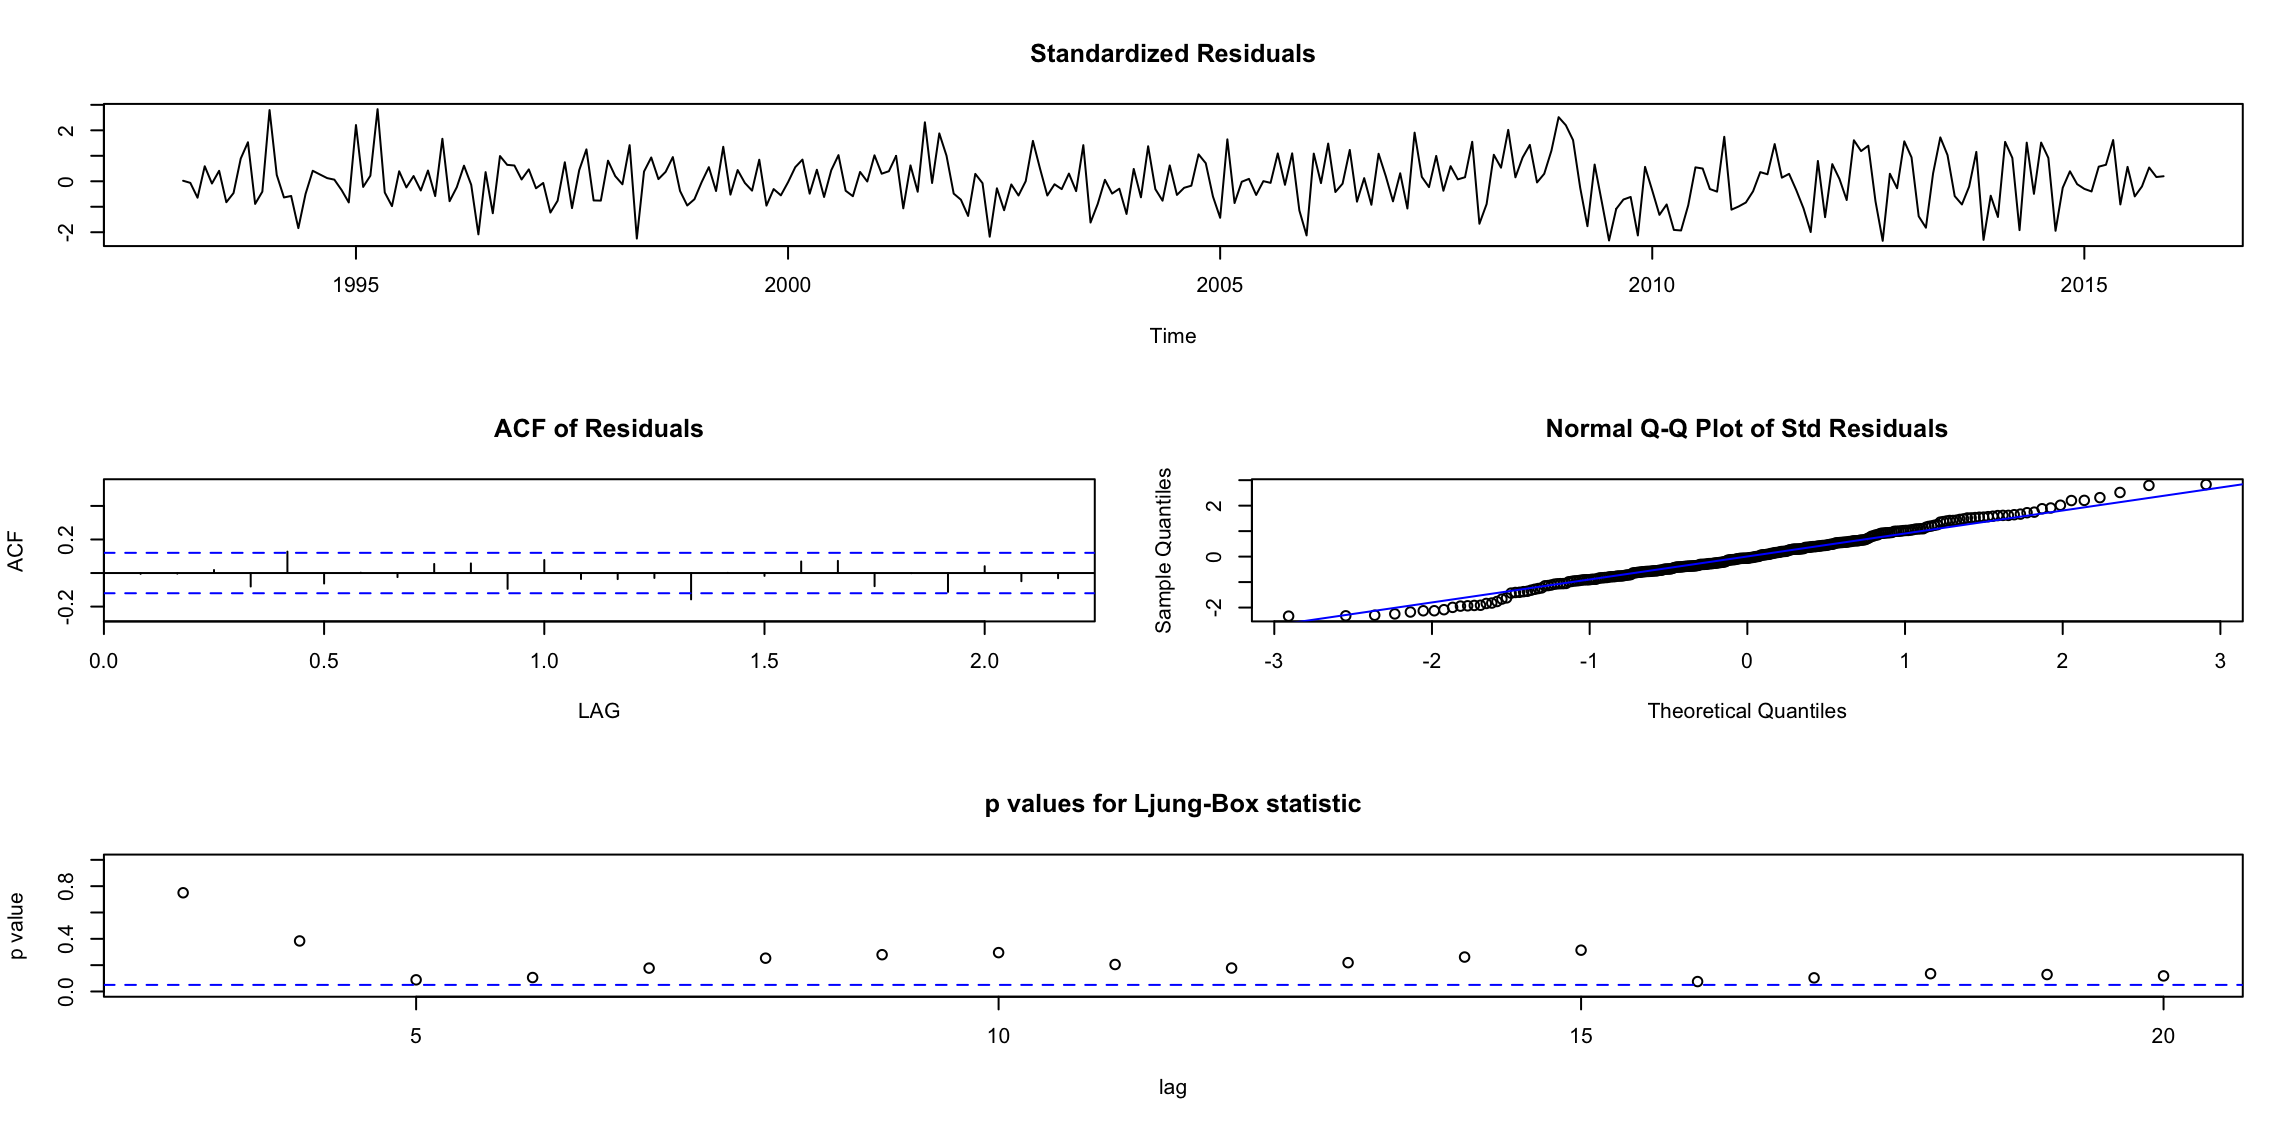
\includegraphics[width=\linewidth]{images/sarima1}
     	\caption*{ARIMA(1,2,1) with no regressors}
     	\label{fig:sarimamod1}
     \end{figure}


    \begin{figure}[htb]
    	\centering
    	\caption{Model 7: Residual Diagnostics}
     	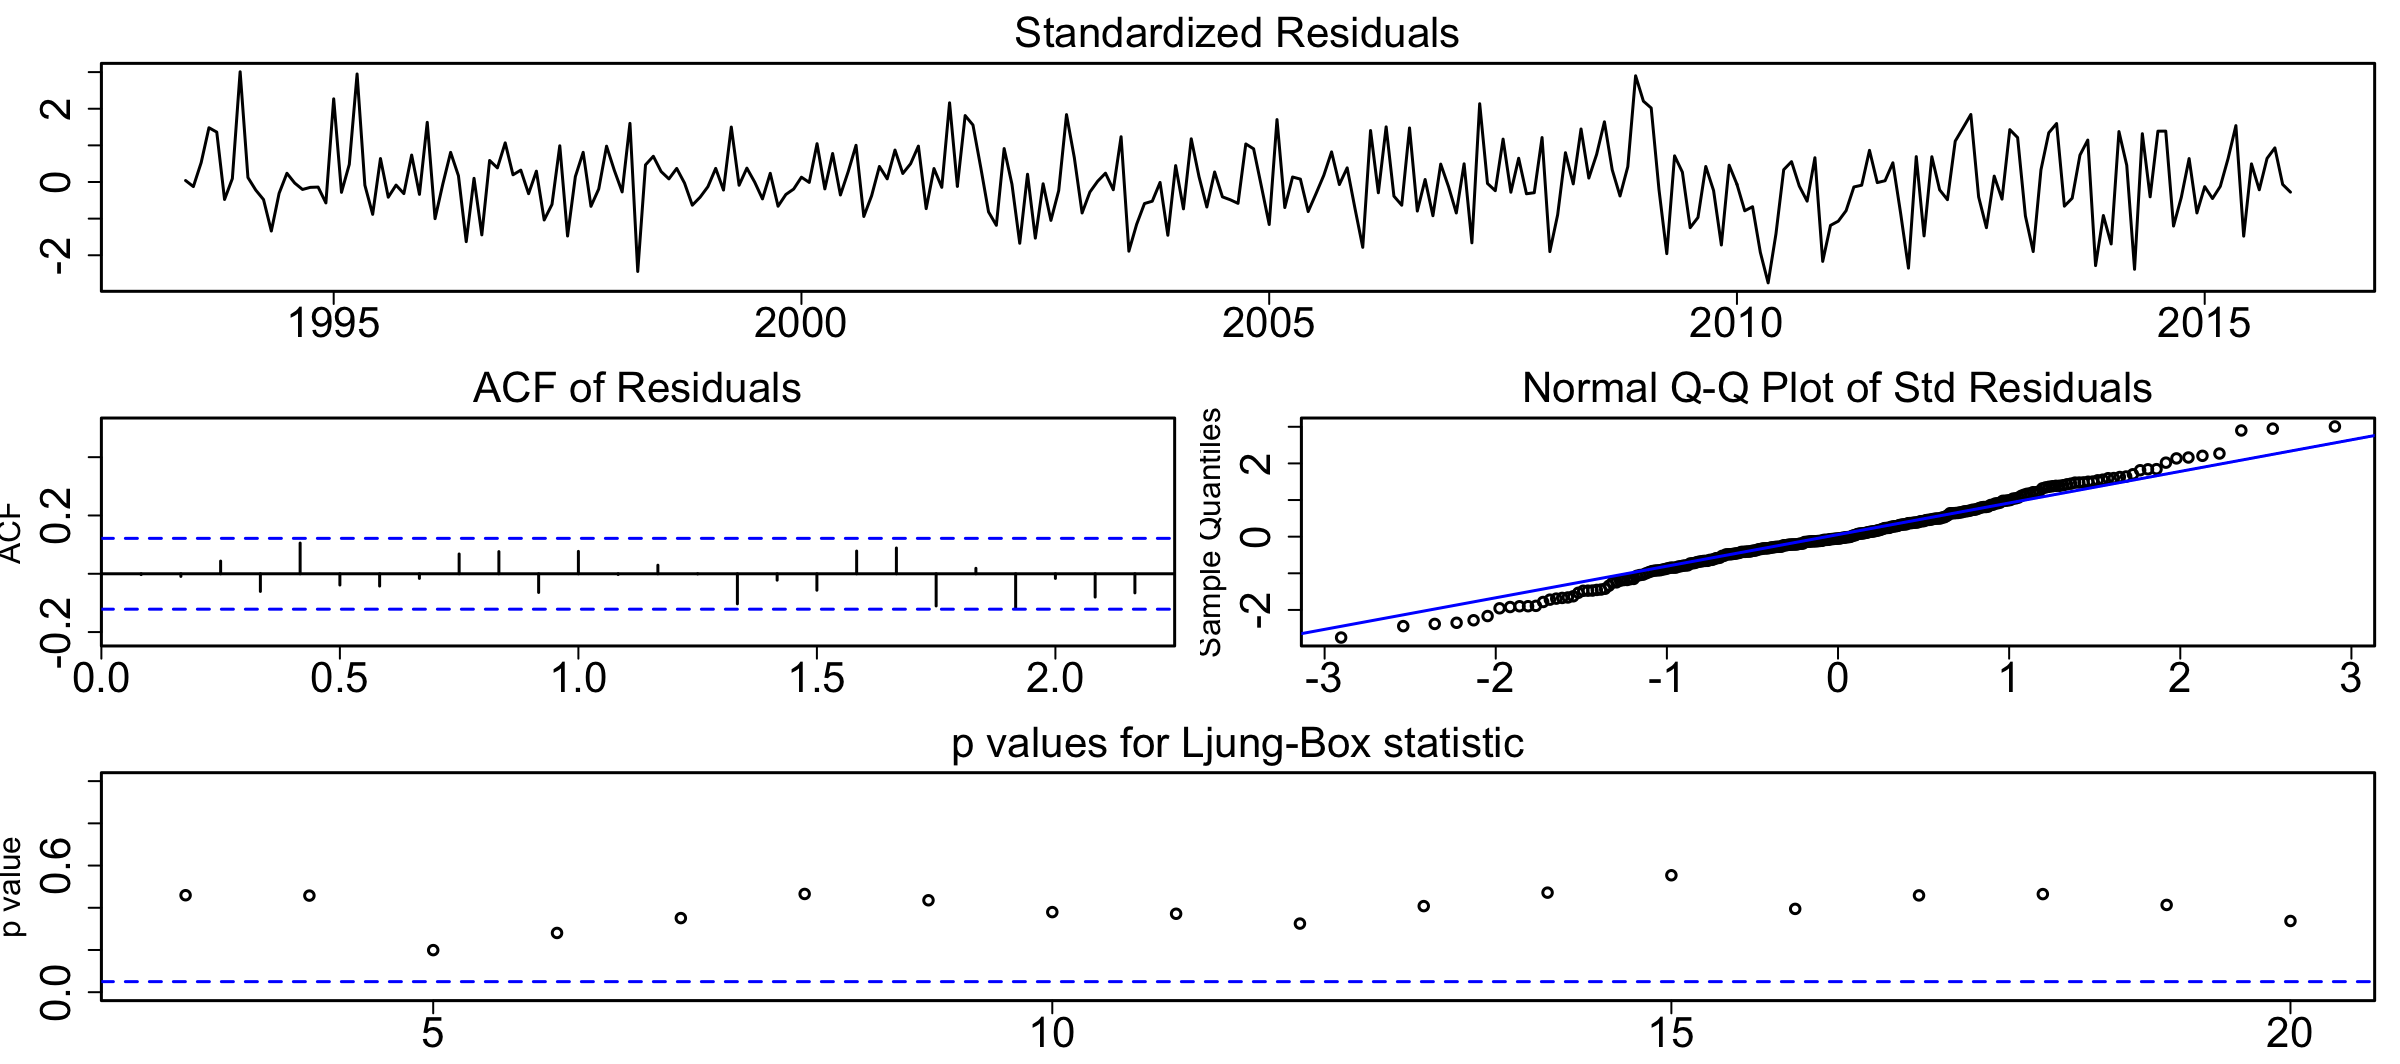
\includegraphics[width=\linewidth]{images/sarima7}
     	\caption*{ARIMA(1,2,1) with lagged regressors}
     	\label{fig:sarimamod7}
     \end{figure}
     
     
     
		Based on the AIC and BIC values, the two ARIMA models that show the most promise are models 1 and 7.  Model 1 includes only the time series data whereas model 7 also includes some lagged versions of the predictors of interest.  The diagnostic plots for these models are shown in Figures \ref{fig:sarimamod1} and \ref{fig:sarimamod7}. Both models show a great deal of promise.  The standardized residuals show no apparent pattern. The ACF of the residuals show no departure from normality. Although the Normal Q-Q plot of the standardized residuals shows some slight departure from normality in the tails, for both models, there is no strong evidence of lack of normality in the residuals  The p-values for the  Ljung-Box statistic are high enough at all plotted lags, so there is no indication of lack of fit in the models. 

      
      \subsubsection{VAR Models}
      % latex table generated in R 3.3.1 by xtable 1.8-2 package
% Sun Jul 24 08:35:48 2016
\begin{table}[htb]
\centering
\caption{VAR models considered}
\label{tab:varchoices}
\begin{tabular}{clllll}
  \hline
 Model & P & Type &  AIC & BIC & Best \\ 
  \hline
1  & 1 & NA  &  -223.67 & -201.97 &  \\ 
  2  & 2 & NA  &   -217.83 & -185.31 &  \\ 
  3  & 1 & Ind  & -256.77 & -231.45 & BIC/AIC \\ 
  4  & 1 & LagX & -216.65 & -195.06 &  \\ 
  5  & 2 & LagX & -212.53 & -180.17 &  \\ 
  6  & 1 & Both  & -245.72 & -220.53 &  \\ 
   \hline
\end{tabular}
\end{table}


      
     Much of the recent literature on modeling unemployment trends has suggesting that vector autoregressive models (VAR) have the capacity to outperform ARIMA models and are widely used by professional forecasters \citep{Meyer2015, Tasci2015, Barnichon2016}. VAR models provide a mechanism for modeling complex, multivariate times series in the absense of a moving average term \citep{Chatfield2001} . The ACF and PACF plots shown in Figures \ref{fig:acfpacf} and \ref{fig:acfpacf2} do not conclusively demonstrate that the moving average term is necessary in this case, therefore we have decided to explore the potential in fitting VAR models to the unemployment data in order to improve the performance of our predictions.  

We started 6 inital VAR models to compare. Models 1, 2, and 3 use the predictors of construction spending and retail sales, without differencing. Model 1 is a VAR(1), model 2 is a VAR(2), and model 3 is a VAR(1) with the regression indicator included as well. Models 4, 5, and 6 repeat the analysis using the differenced version of the predictors. Table \ref{tab:varchoices} shows the AIC and BIC values for each of these models.  

Model 3, the unlagged model with the regression indicator, has the lowest AIC and BIC values.  The diagram of the fit and residuals for model 3 is provided in Figure \ref{fig:varfitmodel3}. The blue line indicates that the actual and predicted values of unemployment are similar in this model. A timeplot of the residuals is consistent with a white noise series. The ACF and PACF of the residuals give no indication of lack of fit. Therefore, we have chosen to retain model 3 to compare with the ARIMA models developed earlier. 


   \begin{figure}[htb]
    	\centering
     	\caption{Model 3 fit and residuals for unemployment}
     	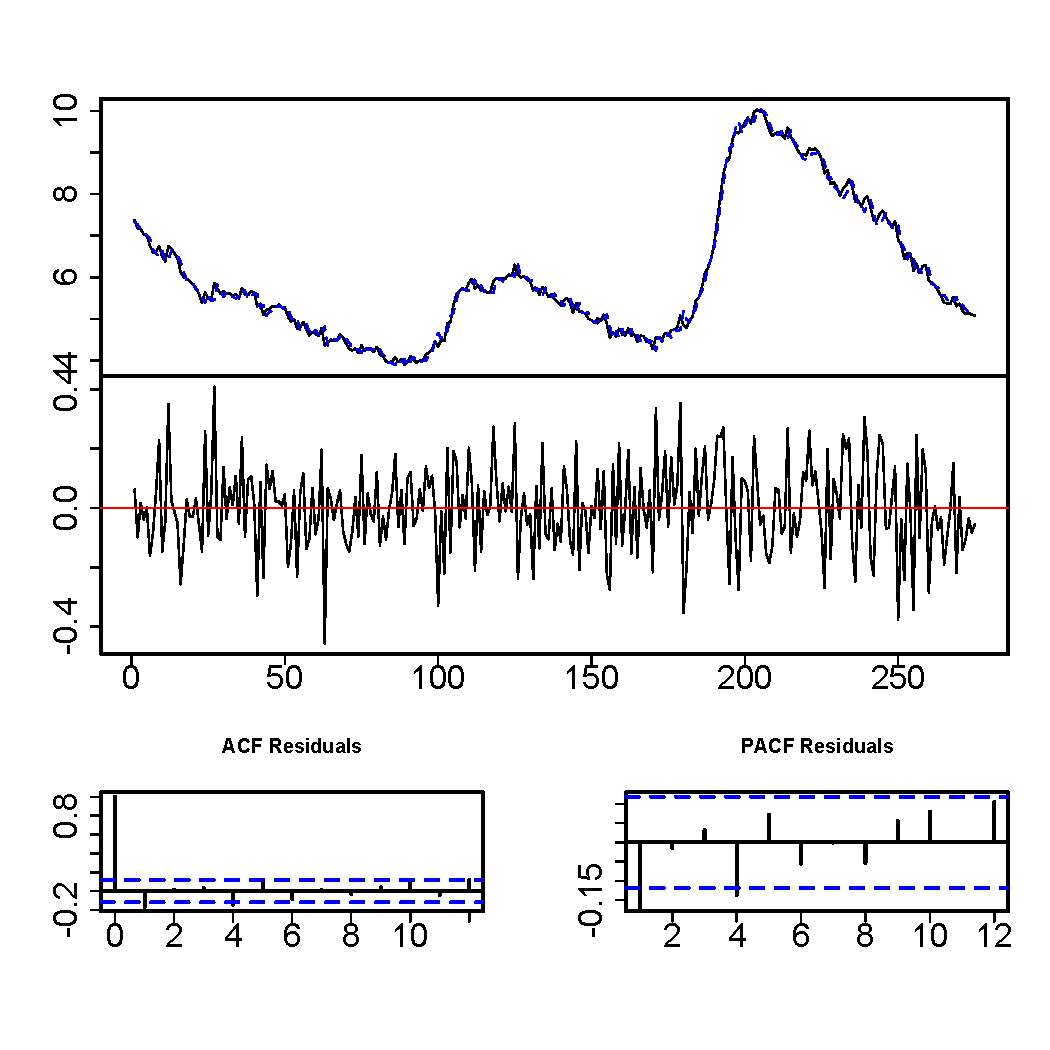
\includegraphics[width=\linewidth]{images/varfitmodel3}
     	\label{fig:varfitmodel3}
 \end{figure}
 
\subsection{Initial Model comparisons}

% latex table generated in R 3.3.1 by xtable 1.8-2 package
% Sun Jul 24 08:35:48 2016
\begin{table}[H]
\centering
\caption{Comparison of ARIMA and VAR models}
\begin{tabular}{llll}
  \hline
Model & Type & AIC & BIC \\ 
  \hline
ARIMA \#1 &Univ ARIMA(1,2,1) &   -212.29 & -201.45  \\ 
ARIMA \#7 & Mult ARIMA(1,2,1)  & -222.45 & -193.69   \\ 
VAR \#3 & VAR(1) & -256.76 & -231.45 \\ 
   \hline
\end{tabular}
\end{table}


In the previous model building process, we retained 3 models for further comparison. ARIMA model 1 is a univariate ARIMA(1,2,1) model without predictors, ARIMA model 7 is a multivariate ARIMA(1,2,1) model with lagged predictors, and 

At first glance the VAR(1) model appears to be the best model.  It has the lowest values of both AIC and BIC.  Of the two ARIMA models the multivariate ARIMA(1,2,1) model has a lower AIC but a higher BIC. However, being a multivariate model, ARIMA \#7 allows us to leverage the additional information provided by indicators of the nature of the economy to refine our predictions about future unemployment rates. 

Since the rate of increasing unemployment is so different from the rate of decreasing unemployment, forcasing can be very difficult without some indicator of whether we are currently in a increasing or decreasing portion of the cycle \citep{Montgomery1998}. For this reason, we have chosen continue our model comparisons with only the two models that include predictors of economic strength. In the next section, we compare the forecasting performance of the best multivariate ARIMA model with best VAR model. These are the multivariate ARIMA(1,2,1) model and the VAR(1) with an indicator variable for recession among its predictors.


\section{Forecasting}

In the initial data setup, the 2016 values were initially excluded to provide a dataset with which to evaluate the performance of our predictions. Short-term predictions from the multivariate ARIMA(1,2,1) model and VAR(1) models were then compared compared with the actual unemployment rates for January 2016 through May 2016. These results were used to create our final model.

\subsection{Multivariate ARIMA(1,2,1)}

   \begin{figure}[htb]
    	\centering
     	\caption{5 month forecast with ARIMA(1,2,1)}
     	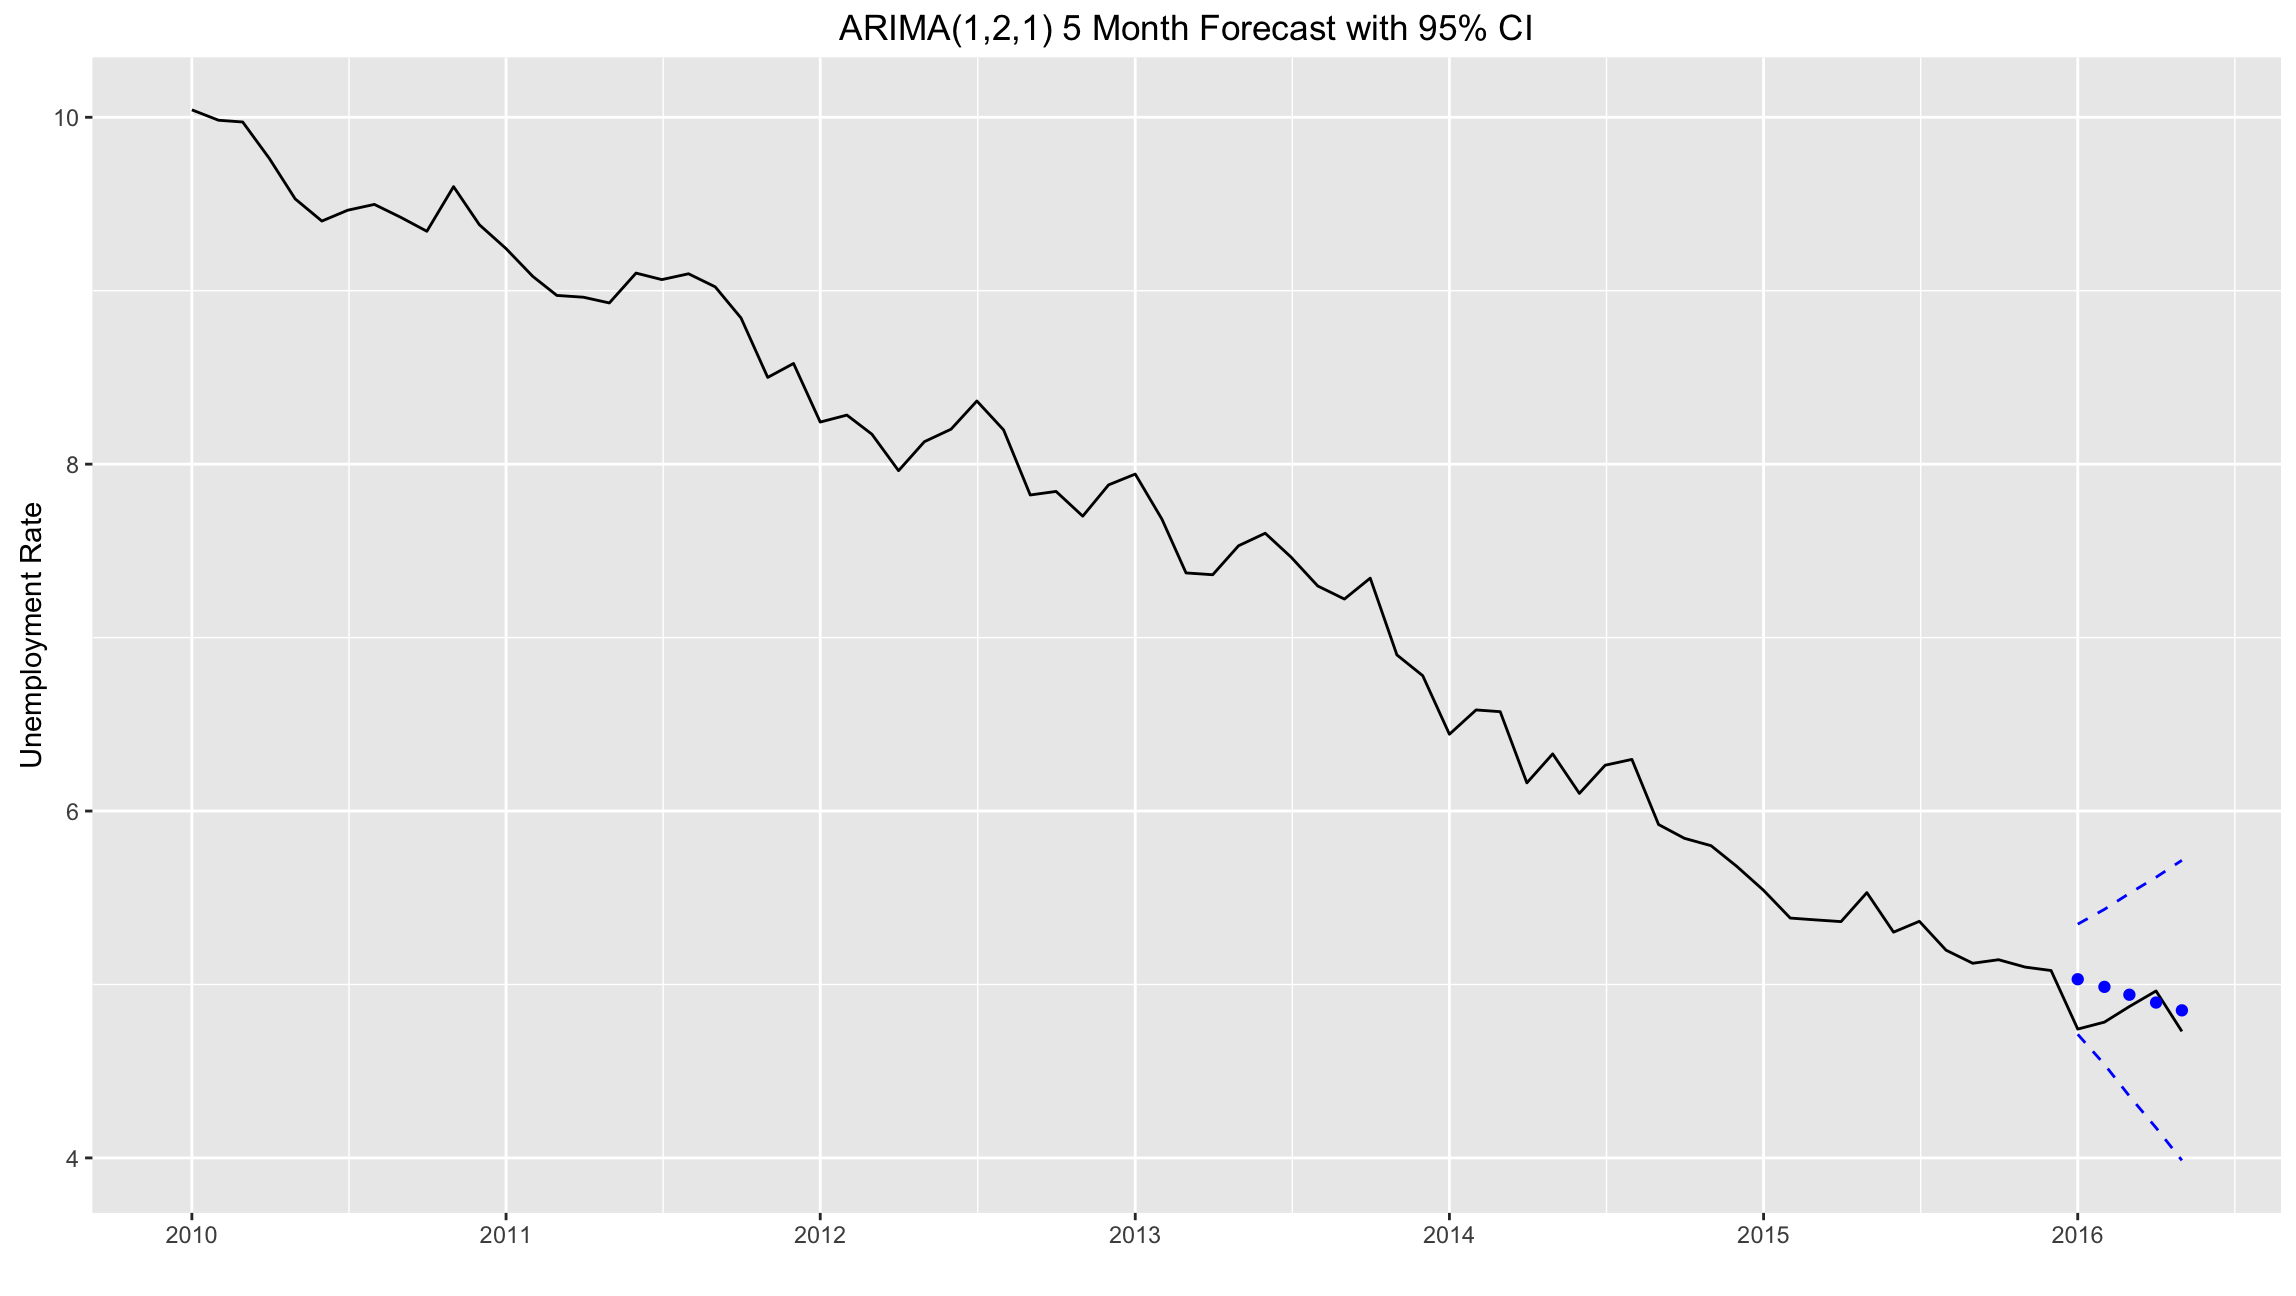
\includegraphics[width=\linewidth]{images/ARIMApred}
     	\label{fig:arimapred}
 \end{figure}

% latex table generated in R 3.2.4 by xtable 1.8-2 package
% Mon Jul 25 11:36:43 2016
\begin{table}[ht]
\centering
\caption{2016 Unemployment Rate Predictions from Multivariate ARIMA(1,2,1)}
\label{tab:arimaforecast}
\begin{tabular}{ccccc}
  \hline
 Month & Observed & Predicted& 95\% CI  & Residual \\ 
  \hline
Jan & 4.74 & 5.03 & (4.71 , 5.35) & -0.29 \\ 
Feb & 4.78 & 4.99 & (4.54 , 5.43) & -0.20 \\ 
Mar & 4.87 & 4.94 & (4.36 , 5.53) & -0.07 \\ 
Apr & 4.96 & 4.90 & (4.17 , 5.62) & 0.07 \\ 
May & 4.73 & 4.85 & (3.99 , 5.72) & -0.12 \\ 
   \hline
\end{tabular}
\end{table}

The unemployment rates for January 2016 to May 2016 were forecast using the Multivariate ARIMA(1,2,1) model, see Table \ref{tab:arimaforecast}.  This model did a good job overall, as all predicted values were within 0.3\% of the actual unemployment rates and entirely inside the confidence bands.  Figure \ref{fig:arimapred} shows the predicted values graphed against the actual unemployment rates. The model predicts a steady decrease in the unemployment rate over the 5 month period.  In general, the ARIMA model provided an overprediction of unemployment rate, except in April-16 when the rate spiked slightly. The confidence bands spread outward rapidly, suggesting an overall pattern of either falling or rising unemployment rate.

\subsection{VAR(1)}

   \begin{figure}[htb]
    	\centering
     	\caption{5 month forecast with VAR(1)}
     	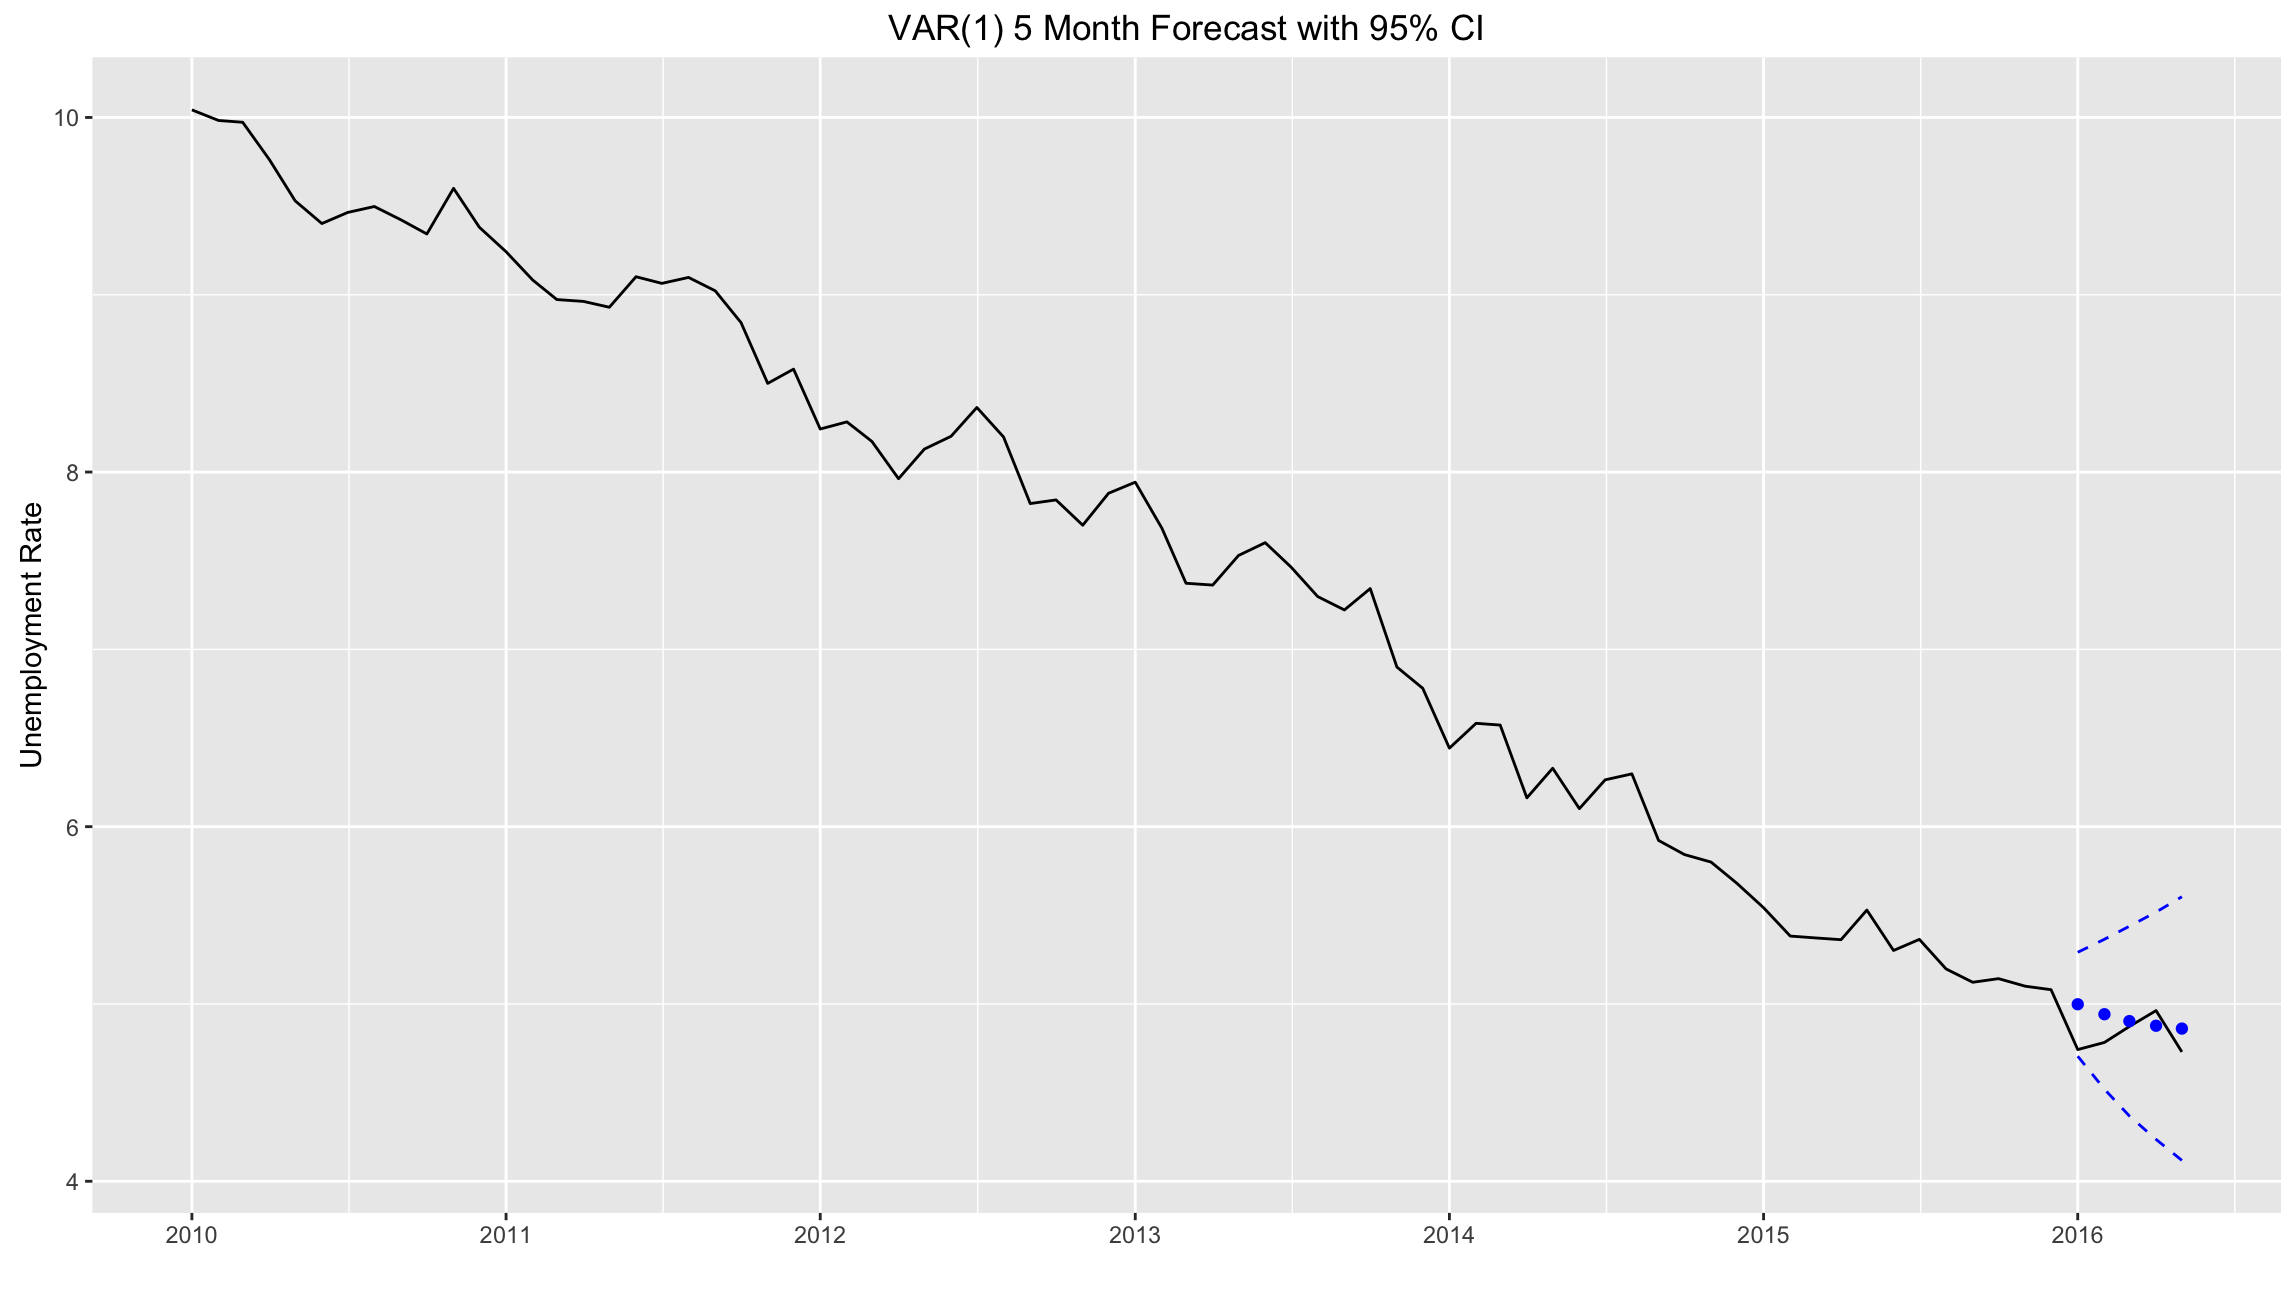
\includegraphics[width=\linewidth]{images/varpred}
     	\label{fig:varpred}
 \end{figure}
 
 % latex table generated in R 3.2.4 by xtable 1.8-2 package
% Mon Jul 25 12:02:02 2016
\begin{table}[ht]
\centering
\small
\caption{2016 Unemployment Rate Predictions from Multivariate VAR(1)}
\label{tab:varforecast}
\begin{tabular}{ccccc}
  \hline
Month & Observed & Predicted& 95\% CI  & Residual \\ 
  \hline
Jan  & 4.74 & 5.00 & (4.71 , 5.29) & -0.26 \\ 
Feb & 4.78 & 4.94 & (4.52 , 5.36) & -0.16 \\ 
Mar  & 4.87 & 4.90 & (4.37 , 5.44) & -0.03 \\ 
Apr & 4.96 & 4.88 & (4.24 , 5.52) & 0.09 \\ 
May & 4.73 & 4.86 & (4.12 , 5.60) & -0.13 \\ 
   \hline
\end{tabular}
\end{table}

The unemployment rates for January 2016 to May 2016 was also forecast using the Var(1) model, see Table \ref{tab:varforecast}.  At first glance the results look very similar to the ARIMA(1,2,1) model. All predicted values were within 0.3\% of the actual unemployment rates and entirely inside the confidence bands.  Figure \ref{fig:varpred} shows the predicted values graphed against the actual unemployment rates. The model predicts a nonlinear decrease in the unemployment rate over the 5 month period, with the rate of decrease slowing over time.  In general, the VAR model also provided an overprediction of unemployment rate, except in April-16. 

 \subsection{Forecast comparisons}
    \begin{figure}[htb]
    	\centering
     	\caption{ARIMA and VAR Model comparison of 3 month forecast}
     	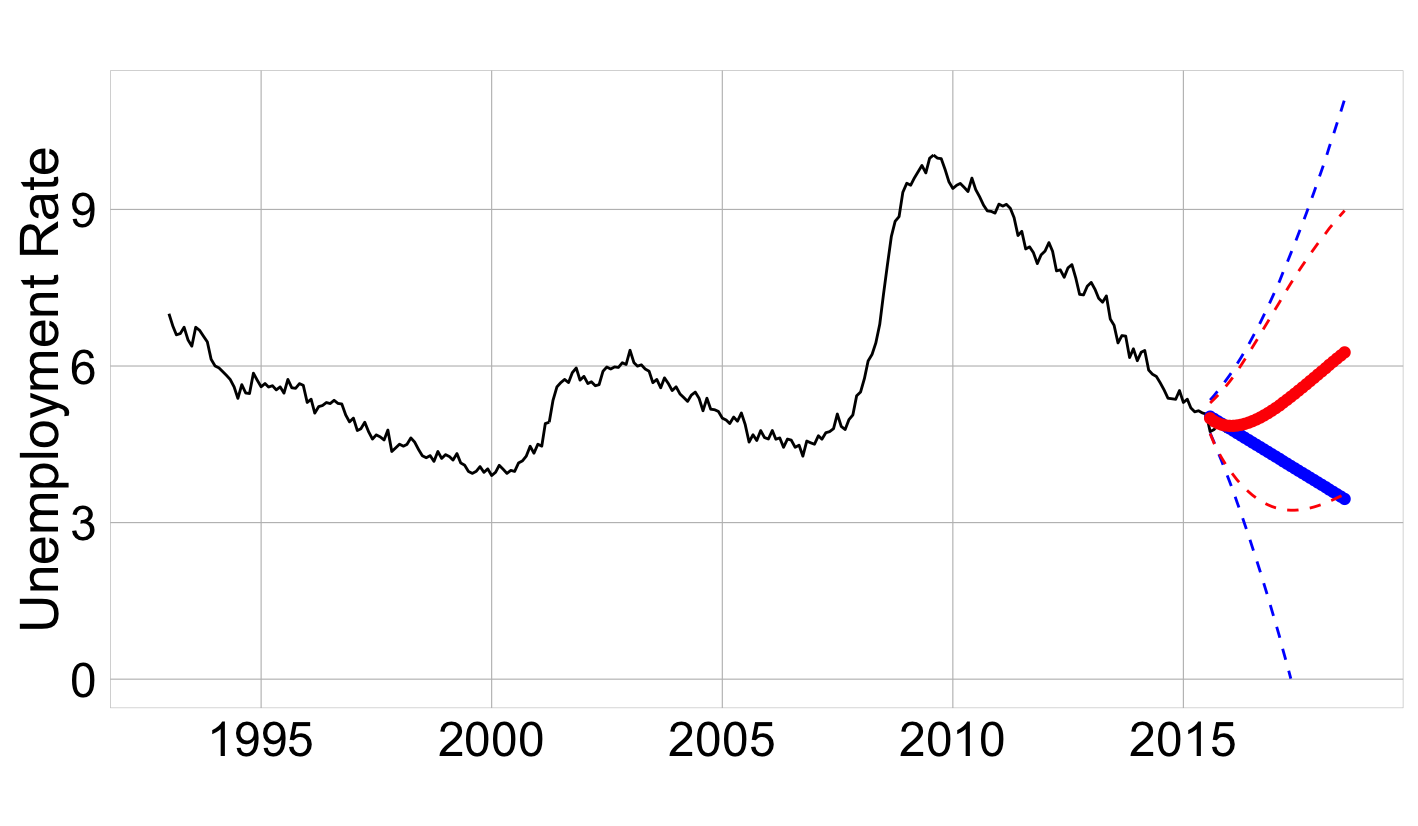
\includegraphics[width=\linewidth]{images/arimavarforecast}
     	\label{fig:arimavarforecast}
 \end{figure}
 
 
      Figure \ref{fig:arimavarforecast} provides a graphical comparison of the two candidate models.  The ARIMA(1, 2, 1) shows a steady, linear decrease of the unemployment rate over time, which is unrealistic in the long term.  The Var model predicts a decrease in unemployment followed by an increase, which is more consistent with actual unemployment patterns. The mean square error from the VAR(1) model (0.0097) is much lower than the mean square error of the ARIMA(1,2,1) model(0.0151). The implication of this is that  the confidence interval of the ARIMA model quickly explodes, suggesting that it may not a good choice for longer term forecasts.
      
In the long run the VAR(1) model seems to provide a much more accurate forecast than the ARIMA(1, 2, 1) model and with much narrower prediction intervals. The complex cyclical nature of unemployment necessitates the use of a more advanced model for longer time periods. However, in the short term VAR(1) is not dramatically more effective than ARIMA(1, 2, 1), suggesting that an VAR(1) model might be overfitting the data in this region. This may be evidence of overfitting, causing more degrees of freedom to be sacraficed than necessary.


 \section{Final model: VAR(1)}

 \subsection{Model estimates} \label{estimates}

The final model chosen was the VAR(1) with construction spending, retail sales, and the recession indicator as predictors.
 The estimates of the coefficients for this model can be found in \ref{tab:estimates}. For this model, all predictors have small p-values, indicating that they add significantly to the model with the other variables included. The positive coefficient for trend suggests that, overall, unemployment has increased over the last 23 years, which is consistent with the overall trend in the time series plot, see Figure \ref{fig:unemployment}. 
 

The coefficient for retail spending is negative, which makes practical sense. If people are spending more money, we would expect that business would have more capital to hire employees. Conversely, people tend to spend less when they are unemployed.  The positive coefficient for construction is a little harder to explain. Higher construction costs tend to be associated with higher unemployment rates, keeping all other variables constant.  This may be is just an artifact of the multivariate nature of the dataset. For a given amount of retail spending, more construction spending is associated with more unemployment. Perhaps this is an indication of the higher cost of resources, when construction materials cost more there is less capital to spend on human resources. Or, maybe it is an indication of income inequality, when unemployment is high builders may cater to wealthier clients to recoup costs. Finally, there is a high positive coefficient for the recession indicator, suggesting that during times of recession unemployment is expected to be higher than in times of economic strength.
 

{\small
\begin{table}[htb]
\centering
\caption{Estimation results for equation VAR(1) model}
\label{tab:estimates}
\begin{tabular}{@{}ccccc@{}}
\toprule
& Estimate & Std. Error & t value & Pr(\(>|t|\))     \\ \midrule
unem.l1      & 0.9752  & 0.0010 & 97.677 & \textless  2e-16 \\
constr.l1    & 0.0043 & 0.0012 & 3.412  & 0.000744 \\
retail.l1    & -0.0059 & 0.0011 & -5.241 & 3.24e-07 \\
recession.l1 & 0.1924  & 0.0318 & 6.051  & 4.80e-09 \\
const        & 0.8438  & 0.2015 & 4.188  & 3.82e-05 \\
trend        & 0.0045  & 0.0009 & 4.759  & 3.17e-06 \\ \bottomrule
\end{tabular}
\end{table}}

The final equation for the VAR(1) model is:
 
 \begin{align*}
  \widehat{\text{U}}\text{nemployment} &= 0.8438_{(0.2015)} +
  0.0045(t)_{(0.0009)}\\ 		
  &+ 0.9752\text{Unemployment}_{t-1 (0.0010)}\\
  &+ 0.0043\text{ConstructionSpend}_{t-1(0.0012)}\\
  &- 0.0059\text{RetailSales}_{t-1(0.0012)}\\
  &+ 0.1924\text{Recession}_{t-1(0.0012)}
  \end{align*} 
 
 \subsection{Model Diagnostics}
 \begin{figure}[hbt]
	\centering
	\caption{VAR Residual Plots}
	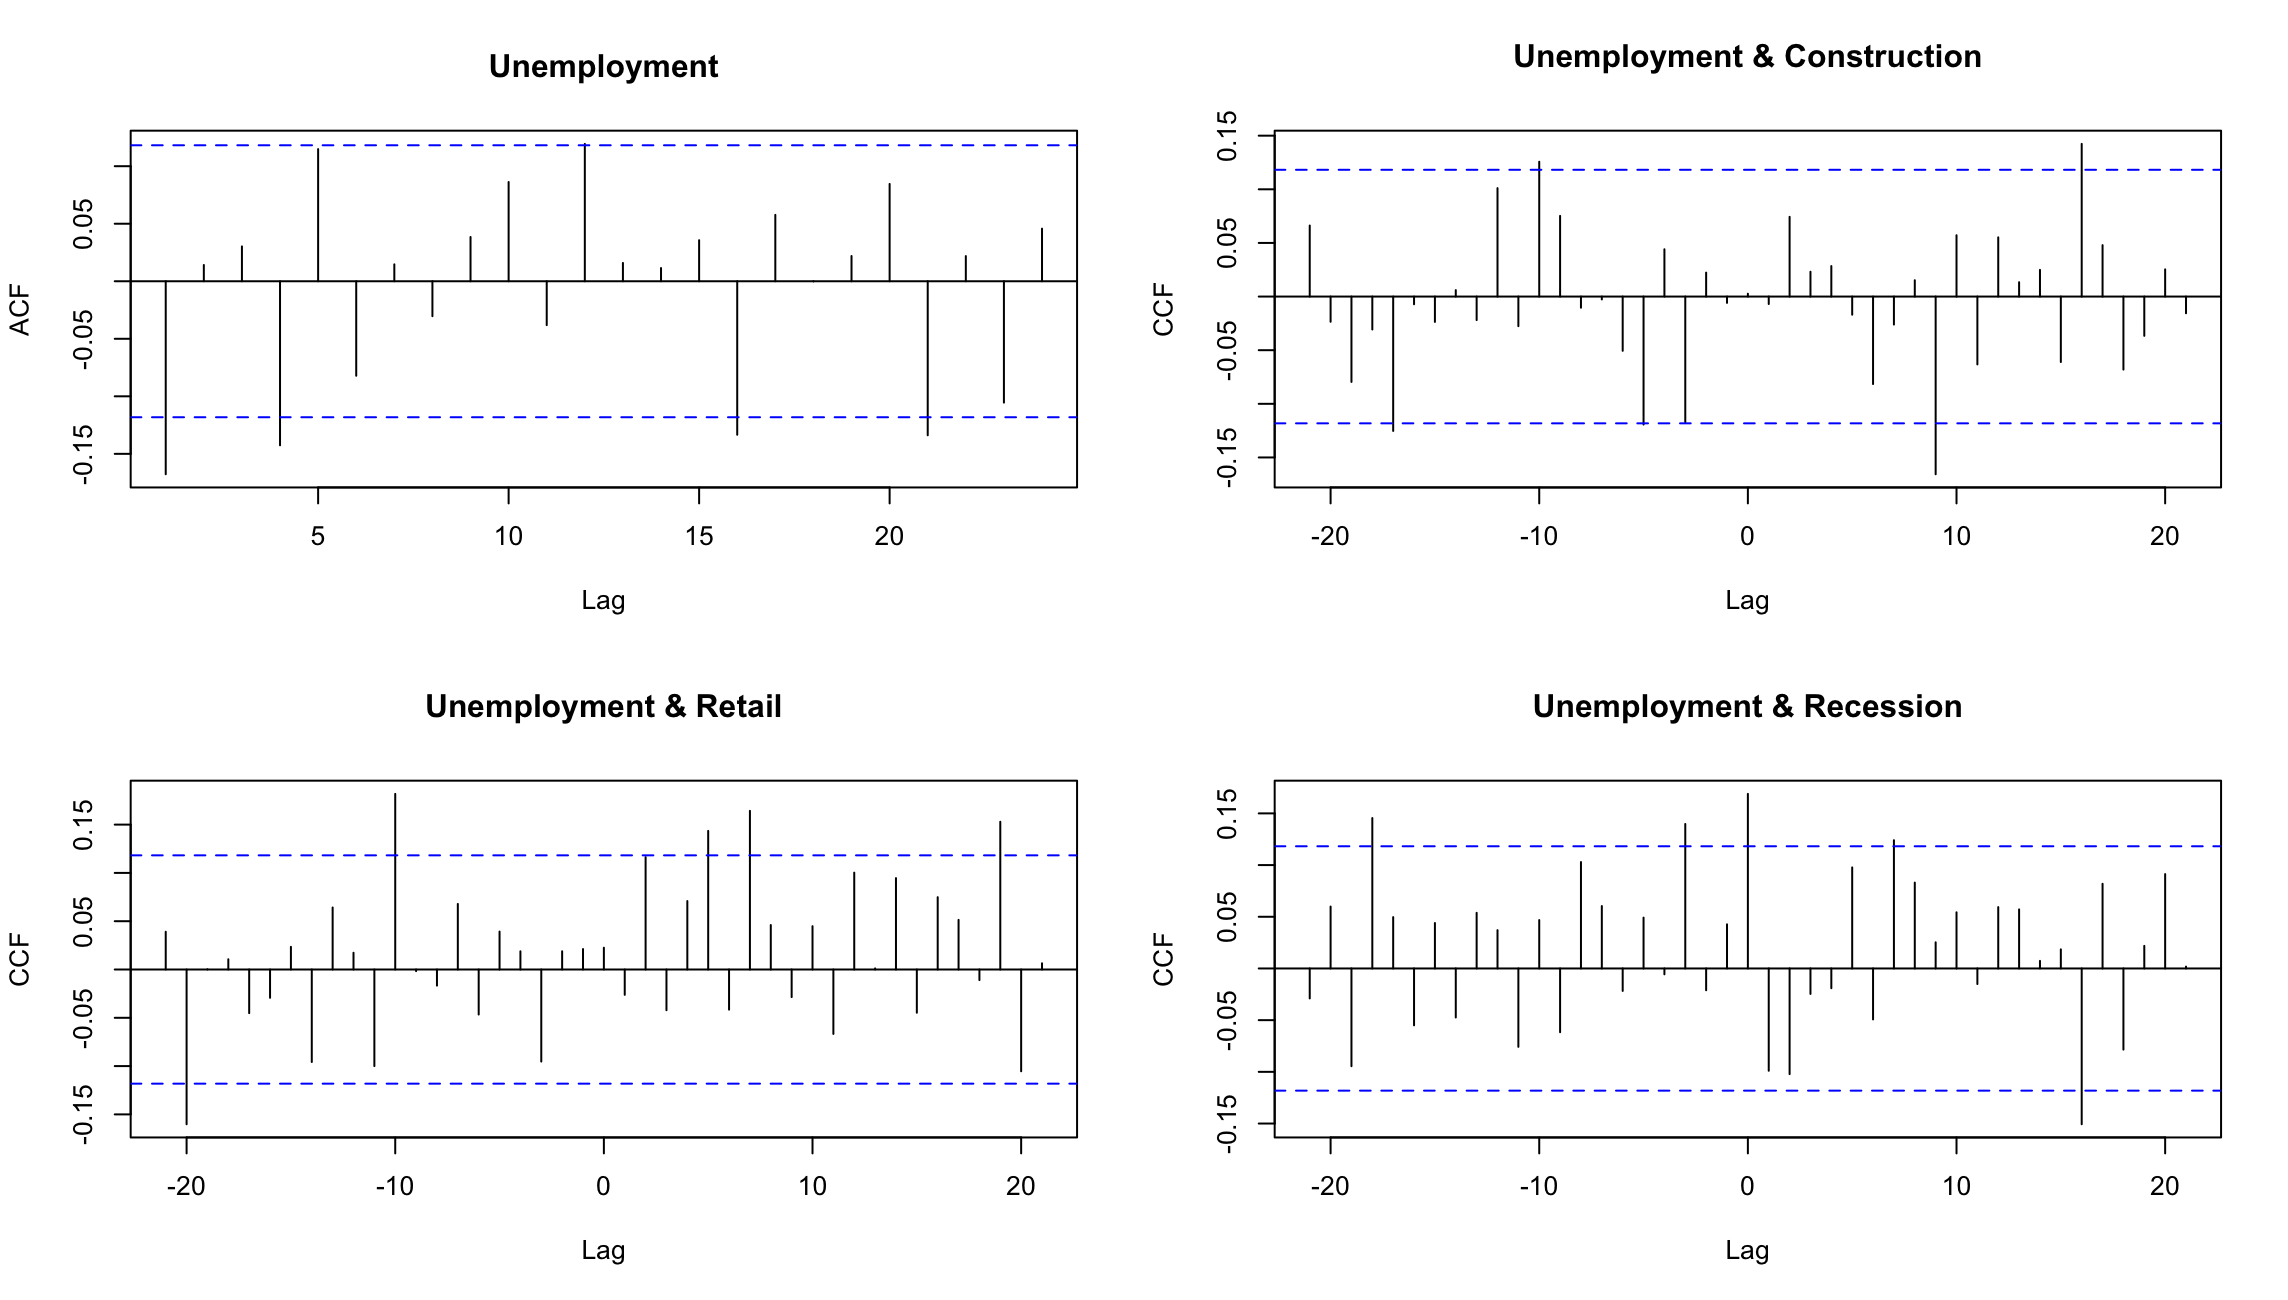
\includegraphics[width=\linewidth]{images/CCFplots}
	\label{fig:CCF}
\end{figure}

Figure \ref{fig:CCF} shows the ACF and the CCF plots for the VAR(1) model of unemployment.  The ACF for the unemployment rate does not indicate any lack of fit for the model. However, the CCF for unemployment vs retail and unemployment vs recession suggest that there may be some left over pattern not captured by the VAR(1) model.   The Portmanteau Test, used to detect model mispecification for multivariate time series \citep{davies1979}, was conducted to test for stationarity in the residuals. Since the Portmanteau statistic was large (\(\chi^2=529.42\), \(df = 176\), \(p < .001\)), we rejected the null hypothesis. There is  strong evidence of nonstationarity in the VAR(1) residuals. This small p-value, along with the graphs above, suggests there is still some dependency left in our model.

\section{Discussion and Implications}

The VAR(1) model given in section \ref{estimates} is a strong model overal. However, given the leftover dependency in the residuals, further investigation may be necessary to create a more reliable model in the long term. Furthermore, there are many economic predictors we did not investigate in this project. Further research should explore these potential explanatory variables in more depth.

We were not able to analyze the effect that presidential transitions had on unemployment.  Visually it appears that each presidential term is accompanied by a sharp increase in unemployment, followed by a slower decline.   This could be investigated using an indicator variable for election year.  Furthermore, it would be interesting to evaluate the impact that party affiliation has on unemployment over time.  Using indicators for presidental party and variables indicating the number of democrats and republicans in congress, we may be able to detect a relationship between unemployment rate and political ideology.

Additionally, a mixed model might be beneficial when modeling complex variables like unemployment rates.  ``Because of the evidence of fractional integration in the unemployment, stationarity and non-linearity issues'' researchers in Croatia utilized a ``multivariate singular spectrum model (MSSA) for modelling unemployment'' \citep{Skare2015}. It would be interesting to explore its potential for use in the U.S. which has a significantly larger economy and population.  Or, perhaps we could create a model that somehow combining the simplicity of the ARIMA models for short term predictions with the more complex structure needed for the long term. After further development, the model should be tested on the other unemployment rates, such as industry specific or local uneemployment rates.

\subsection{Conclusion}

Unemployment in the United States is an issue that is complex and socially meaningful. Recent research has explored the use of VAR models and worker flow data to predict the direction of unemployment in the short term. This project has attempted to predict unemployment rates using other economic indicators, including spending and recession time period. While the model created was strong, with relatively precise short term accuracy, it could benefit from further refinement. Future research in this area should include more variables, spectral analysis, and a mixed model approach. 

%----------------------------------------------------------------------------------------
%	REFERENCE LIST
%----------------------------------------------------------------------------------------

\begin{flushleft}
\bibliography{main} % refers to our bibliography
\end{flushleft}
 \section*{Appendix}
 \appendix
 \section*{Project contributions}
 \begin{itemize}
 	\item Joseph Blubaugh
 		\begin{itemize}
 			\item Plots
 			\item Data Prep
 			\item Code Management
 			\item Model refinement
 		\end{itemize}
 		
 	\item Sean Roberson
 	 		\begin{itemize}
 			\item Presentor
 			\item Key talking points
 			\item Model clarification
 			\item Literature
 		\end{itemize}
 	
	\item Akarshan Puri
			\begin{itemize}
 			\item Model selection
 			\item Model diagnostics
 			\item Model fitting
 		\end{itemize}
 	
 	\item Alison Shelton
 			\begin{itemize}
 				\item \LaTeX \ code management
 				\item Writing
 				\item Literature
 			\end{itemize}
	
	\item Travis Lilley
			 \begin{itemize}
			 \item Model building
			 \item Model fitting
			 \item Model diagnostics
			 \item Abstract
			 \end{itemize}

	\item{Bo Pang}
		\begin{itemize}
					\item Model building
		 			\item Model diagnostics
		 			\item Model fitting
		\end{itemize}
 \end{itemize}

Please note, this project was done in a collaborative fashion using GitHub as a tool for collaborative coding and writing. Therefore, the above list of contributions is only a rough estimate of how the workload was distributed. Each member worked on every component.  While the project was small we used Overleaf for collaborative writing, as it grew changes were pushed to GitHub.  Literature references were shared on GitHub and using Mendeley.  

It is particularly important to note that once an intial file was placed on the repository, all members had access to and modified each other's code. We believe this brings strength to our project but it makes it difficult to definitively state who contributed to each portion in a consice manner.

For  the R-code used in this project and more information about our project management process please see \url{https://github.com/JestonBlu/STAT626_PROJECT}.
\end{document}
